\documentclass{article}
\usepackage{iclr2027_conference,times}
%%%%% NEW MATH DEFINITIONS %%%%%

\usepackage{amsmath,amsfonts,bm}

% Mark sections of captions for referring to divisions of figures
\newcommand{\figleft}{{\em (Left)}}
\newcommand{\figcenter}{{\em (Center)}}
\newcommand{\figright}{{\em (Right)}}
\newcommand{\figtop}{{\em (Top)}}
\newcommand{\figbottom}{{\em (Bottom)}}
\newcommand{\captiona}{{\em (a)}}
\newcommand{\captionb}{{\em (b)}}
\newcommand{\captionc}{{\em (c)}}
\newcommand{\captiond}{{\em (d)}}

% Highlight a newly defined term
\newcommand{\newterm}[1]{{\bf #1}}


% Figure reference, lower-case.
\def\figref#1{figure~\ref{#1}}
% Figure reference, capital. For start of sentence
\def\Figref#1{Figure~\ref{#1}}
\def\twofigref#1#2{figures \ref{#1} and \ref{#2}}
\def\quadfigref#1#2#3#4{figures \ref{#1}, \ref{#2}, \ref{#3} and \ref{#4}}
% Section reference, lower-case.
\def\secref#1{section~\ref{#1}}
% Section reference, capital.
\def\Secref#1{Section~\ref{#1}}
% Reference to two sections.
\def\twosecrefs#1#2{sections \ref{#1} and \ref{#2}}
% Reference to three sections.
\def\secrefs#1#2#3{sections \ref{#1}, \ref{#2} and \ref{#3}}
% Reference to an equation, lower-case.
\def\eqref#1{equation~\ref{#1}}
% Reference to an equation, upper case
\def\Eqref#1{Equation~\ref{#1}}
% A raw reference to an equation---avoid using if possible
\def\plaineqref#1{\ref{#1}}
% Reference to a chapter, lower-case.
\def\chapref#1{chapter~\ref{#1}}
% Reference to an equation, upper case.
\def\Chapref#1{Chapter~\ref{#1}}
% Reference to a range of chapters
\def\rangechapref#1#2{chapters\ref{#1}--\ref{#2}}
% Reference to an algorithm, lower-case.
\def\algref#1{algorithm~\ref{#1}}
% Reference to an algorithm, upper case.
\def\Algref#1{Algorithm~\ref{#1}}
\def\twoalgref#1#2{algorithms \ref{#1} and \ref{#2}}
\def\Twoalgref#1#2{Algorithms \ref{#1} and \ref{#2}}
% Reference to a part, lower case
\def\partref#1{part~\ref{#1}}
% Reference to a part, upper case
\def\Partref#1{Part~\ref{#1}}
\def\twopartref#1#2{parts \ref{#1} and \ref{#2}}

\def\ceil#1{\lceil #1 \rceil}
\def\floor#1{\lfloor #1 \rfloor}
\def\1{\bm{1}}
\newcommand{\train}{\mathcal{D}}
\newcommand{\valid}{\mathcal{D_{\mathrm{valid}}}}
\newcommand{\test}{\mathcal{D_{\mathrm{test}}}}

\def\eps{{\epsilon}}


% Random variables
\def\reta{{\textnormal{$\eta$}}}
\def\ra{{\textnormal{a}}}
\def\rb{{\textnormal{b}}}
\def\rc{{\textnormal{c}}}
\def\rd{{\textnormal{d}}}
\def\re{{\textnormal{e}}}
\def\rf{{\textnormal{f}}}
\def\rg{{\textnormal{g}}}
\def\rh{{\textnormal{h}}}
\def\ri{{\textnormal{i}}}
\def\rj{{\textnormal{j}}}
\def\rk{{\textnormal{k}}}
\def\rl{{\textnormal{l}}}
% rm is already a command, just don't name any random variables m
\def\rn{{\textnormal{n}}}
\def\ro{{\textnormal{o}}}
\def\rp{{\textnormal{p}}}
\def\rq{{\textnormal{q}}}
\def\rr{{\textnormal{r}}}
\def\rs{{\textnormal{s}}}
\def\rt{{\textnormal{t}}}
\def\ru{{\textnormal{u}}}
\def\rv{{\textnormal{v}}}
\def\rw{{\textnormal{w}}}
\def\rx{{\textnormal{x}}}
\def\ry{{\textnormal{y}}}
\def\rz{{\textnormal{z}}}

% Random vectors
\def\rvepsilon{{\mathbf{\epsilon}}}
\def\rvtheta{{\mathbf{\theta}}}
\def\rva{{\mathbf{a}}}
\def\rvb{{\mathbf{b}}}
\def\rvc{{\mathbf{c}}}
\def\rvd{{\mathbf{d}}}
\def\rve{{\mathbf{e}}}
\def\rvf{{\mathbf{f}}}
\def\rvg{{\mathbf{g}}}
\def\rvh{{\mathbf{h}}}
\def\rvu{{\mathbf{i}}}
\def\rvj{{\mathbf{j}}}
\def\rvk{{\mathbf{k}}}
\def\rvl{{\mathbf{l}}}
\def\rvm{{\mathbf{m}}}
\def\rvn{{\mathbf{n}}}
\def\rvo{{\mathbf{o}}}
\def\rvp{{\mathbf{p}}}
\def\rvq{{\mathbf{q}}}
\def\rvr{{\mathbf{r}}}
\def\rvs{{\mathbf{s}}}
\def\rvt{{\mathbf{t}}}
\def\rvu{{\mathbf{u}}}
\def\rvv{{\mathbf{v}}}
\def\rvw{{\mathbf{w}}}
\def\rvx{{\mathbf{x}}}
\def\rvy{{\mathbf{y}}}
\def\rvz{{\mathbf{z}}}

% Elements of random vectors
\def\erva{{\textnormal{a}}}
\def\ervb{{\textnormal{b}}}
\def\ervc{{\textnormal{c}}}
\def\ervd{{\textnormal{d}}}
\def\erve{{\textnormal{e}}}
\def\ervf{{\textnormal{f}}}
\def\ervg{{\textnormal{g}}}
\def\ervh{{\textnormal{h}}}
\def\ervi{{\textnormal{i}}}
\def\ervj{{\textnormal{j}}}
\def\ervk{{\textnormal{k}}}
\def\ervl{{\textnormal{l}}}
\def\ervm{{\textnormal{m}}}
\def\ervn{{\textnormal{n}}}
\def\ervo{{\textnormal{o}}}
\def\ervp{{\textnormal{p}}}
\def\ervq{{\textnormal{q}}}
\def\ervr{{\textnormal{r}}}
\def\ervs{{\textnormal{s}}}
\def\ervt{{\textnormal{t}}}
\def\ervu{{\textnormal{u}}}
\def\ervv{{\textnormal{v}}}
\def\ervw{{\textnormal{w}}}
\def\ervx{{\textnormal{x}}}
\def\ervy{{\textnormal{y}}}
\def\ervz{{\textnormal{z}}}

% Random matrices
\def\rmA{{\mathbf{A}}}
\def\rmB{{\mathbf{B}}}
\def\rmC{{\mathbf{C}}}
\def\rmD{{\mathbf{D}}}
\def\rmE{{\mathbf{E}}}
\def\rmF{{\mathbf{F}}}
\def\rmG{{\mathbf{G}}}
\def\rmH{{\mathbf{H}}}
\def\rmI{{\mathbf{I}}}
\def\rmJ{{\mathbf{J}}}
\def\rmK{{\mathbf{K}}}
\def\rmL{{\mathbf{L}}}
\def\rmM{{\mathbf{M}}}
\def\rmN{{\mathbf{N}}}
\def\rmO{{\mathbf{O}}}
\def\rmP{{\mathbf{P}}}
\def\rmQ{{\mathbf{Q}}}
\def\rmR{{\mathbf{R}}}
\def\rmS{{\mathbf{S}}}
\def\rmT{{\mathbf{T}}}
\def\rmU{{\mathbf{U}}}
\def\rmV{{\mathbf{V}}}
\def\rmW{{\mathbf{W}}}
\def\rmX{{\mathbf{X}}}
\def\rmY{{\mathbf{Y}}}
\def\rmZ{{\mathbf{Z}}}

% Elements of random matrices
\def\ermA{{\textnormal{A}}}
\def\ermB{{\textnormal{B}}}
\def\ermC{{\textnormal{C}}}
\def\ermD{{\textnormal{D}}}
\def\ermE{{\textnormal{E}}}
\def\ermF{{\textnormal{F}}}
\def\ermG{{\textnormal{G}}}
\def\ermH{{\textnormal{H}}}
\def\ermI{{\textnormal{I}}}
\def\ermJ{{\textnormal{J}}}
\def\ermK{{\textnormal{K}}}
\def\ermL{{\textnormal{L}}}
\def\ermM{{\textnormal{M}}}
\def\ermN{{\textnormal{N}}}
\def\ermO{{\textnormal{O}}}
\def\ermP{{\textnormal{P}}}
\def\ermQ{{\textnormal{Q}}}
\def\ermR{{\textnormal{R}}}
\def\ermS{{\textnormal{S}}}
\def\ermT{{\textnormal{T}}}
\def\ermU{{\textnormal{U}}}
\def\ermV{{\textnormal{V}}}
\def\ermW{{\textnormal{W}}}
\def\ermX{{\textnormal{X}}}
\def\ermY{{\textnormal{Y}}}
\def\ermZ{{\textnormal{Z}}}

% Vectors
\def\vzero{{\bm{0}}}
\def\vone{{\bm{1}}}
\def\vmu{{\bm{\mu}}}
\def\vtheta{{\bm{\theta}}}
\def\va{{\bm{a}}}
\def\vb{{\bm{b}}}
\def\vc{{\bm{c}}}
\def\vd{{\bm{d}}}
\def\ve{{\bm{e}}}
\def\vf{{\bm{f}}}
\def\vg{{\bm{g}}}
\def\vh{{\bm{h}}}
\def\vi{{\bm{i}}}
\def\vj{{\bm{j}}}
\def\vk{{\bm{k}}}
\def\vl{{\bm{l}}}
\def\vm{{\bm{m}}}
\def\vn{{\bm{n}}}
\def\vo{{\bm{o}}}
\def\vp{{\bm{p}}}
\def\vq{{\bm{q}}}
\def\vr{{\bm{r}}}
\def\vs{{\bm{s}}}
\def\vt{{\bm{t}}}
\def\vu{{\bm{u}}}
\def\vv{{\bm{v}}}
\def\vw{{\bm{w}}}
\def\vx{{\bm{x}}}
\def\vy{{\bm{y}}}
\def\vz{{\bm{z}}}

% Elements of vectors
\def\evalpha{{\alpha}}
\def\evbeta{{\beta}}
\def\evepsilon{{\epsilon}}
\def\evlambda{{\lambda}}
\def\evomega{{\omega}}
\def\evmu{{\mu}}
\def\evpsi{{\psi}}
\def\evsigma{{\sigma}}
\def\evtheta{{\theta}}
\def\eva{{a}}
\def\evb{{b}}
\def\evc{{c}}
\def\evd{{d}}
\def\eve{{e}}
\def\evf{{f}}
\def\evg{{g}}
\def\evh{{h}}
\def\evi{{i}}
\def\evj{{j}}
\def\evk{{k}}
\def\evl{{l}}
\def\evm{{m}}
\def\evn{{n}}
\def\evo{{o}}
\def\evp{{p}}
\def\evq{{q}}
\def\evr{{r}}
\def\evs{{s}}
\def\evt{{t}}
\def\evu{{u}}
\def\evv{{v}}
\def\evw{{w}}
\def\evx{{x}}
\def\evy{{y}}
\def\evz{{z}}

% Matrix
\def\mA{{\bm{A}}}
\def\mB{{\bm{B}}}
\def\mC{{\bm{C}}}
\def\mD{{\bm{D}}}
\def\mE{{\bm{E}}}
\def\mF{{\bm{F}}}
\def\mG{{\bm{G}}}
\def\mH{{\bm{H}}}
\def\mI{{\bm{I}}}
\def\mJ{{\bm{J}}}
\def\mK{{\bm{K}}}
\def\mL{{\bm{L}}}
\def\mM{{\bm{M}}}
\def\mN{{\bm{N}}}
\def\mO{{\bm{O}}}
\def\mP{{\bm{P}}}
\def\mQ{{\bm{Q}}}
\def\mR{{\bm{R}}}
\def\mS{{\bm{S}}}
\def\mT{{\bm{T}}}
\def\mU{{\bm{U}}}
\def\mV{{\bm{V}}}
\def\mW{{\bm{W}}}
\def\mX{{\bm{X}}}
\def\mY{{\bm{Y}}}
\def\mZ{{\bm{Z}}}
\def\mBeta{{\bm{\beta}}}
\def\mPhi{{\bm{\Phi}}}
\def\mLambda{{\bm{\Lambda}}}
\def\mSigma{{\bm{\Sigma}}}

% Tensor
\DeclareMathAlphabet{\mathsfit}{\encodingdefault}{\sfdefault}{m}{sl}
\SetMathAlphabet{\mathsfit}{bold}{\encodingdefault}{\sfdefault}{bx}{n}
\newcommand{\tens}[1]{\bm{\mathsfit{#1}}}
\def\tA{{\tens{A}}}
\def\tB{{\tens{B}}}
\def\tC{{\tens{C}}}
\def\tD{{\tens{D}}}
\def\tE{{\tens{E}}}
\def\tF{{\tens{F}}}
\def\tG{{\tens{G}}}
\def\tH{{\tens{H}}}
\def\tI{{\tens{I}}}
\def\tJ{{\tens{J}}}
\def\tK{{\tens{K}}}
\def\tL{{\tens{L}}}
\def\tM{{\tens{M}}}
\def\tN{{\tens{N}}}
\def\tO{{\tens{O}}}
\def\tP{{\tens{P}}}
\def\tQ{{\tens{Q}}}
\def\tR{{\tens{R}}}
\def\tS{{\tens{S}}}
\def\tT{{\tens{T}}}
\def\tU{{\tens{U}}}
\def\tV{{\tens{V}}}
\def\tW{{\tens{W}}}
\def\tX{{\tens{X}}}
\def\tY{{\tens{Y}}}
\def\tZ{{\tens{Z}}}


% Graph
\def\gA{{\mathcal{A}}}
\def\gB{{\mathcal{B}}}
\def\gC{{\mathcal{C}}}
\def\gD{{\mathcal{D}}}
\def\gE{{\mathcal{E}}}
\def\gF{{\mathcal{F}}}
\def\gG{{\mathcal{G}}}
\def\gH{{\mathcal{H}}}
\def\gI{{\mathcal{I}}}
\def\gJ{{\mathcal{J}}}
\def\gK{{\mathcal{K}}}
\def\gL{{\mathcal{L}}}
\def\gM{{\mathcal{M}}}
\def\gN{{\mathcal{N}}}
\def\gO{{\mathcal{O}}}
\def\gP{{\mathcal{P}}}
\def\gQ{{\mathcal{Q}}}
\def\gR{{\mathcal{R}}}
\def\gS{{\mathcal{S}}}
\def\gT{{\mathcal{T}}}
\def\gU{{\mathcal{U}}}
\def\gV{{\mathcal{V}}}
\def\gW{{\mathcal{W}}}
\def\gX{{\mathcal{X}}}
\def\gY{{\mathcal{Y}}}
\def\gZ{{\mathcal{Z}}}

% Sets
\def\sA{{\mathbb{A}}}
\def\sB{{\mathbb{B}}}
\def\sC{{\mathbb{C}}}
\def\sD{{\mathbb{D}}}
% Don't use a set called E, because this would be the same as our symbol
% for expectation.
\def\sF{{\mathbb{F}}}
\def\sG{{\mathbb{G}}}
\def\sH{{\mathbb{H}}}
\def\sI{{\mathbb{I}}}
\def\sJ{{\mathbb{J}}}
\def\sK{{\mathbb{K}}}
\def\sL{{\mathbb{L}}}
\def\sM{{\mathbb{M}}}
\def\sN{{\mathbb{N}}}
\def\sO{{\mathbb{O}}}
\def\sP{{\mathbb{P}}}
\def\sQ{{\mathbb{Q}}}
\def\sR{{\mathbb{R}}}
\def\sS{{\mathbb{S}}}
\def\sT{{\mathbb{T}}}
\def\sU{{\mathbb{U}}}
\def\sV{{\mathbb{V}}}
\def\sW{{\mathbb{W}}}
\def\sX{{\mathbb{X}}}
\def\sY{{\mathbb{Y}}}
\def\sZ{{\mathbb{Z}}}

% Entries of a matrix
\def\emLambda{{\Lambda}}
\def\emA{{A}}
\def\emB{{B}}
\def\emC{{C}}
\def\emD{{D}}
\def\emE{{E}}
\def\emF{{F}}
\def\emG{{G}}
\def\emH{{H}}
\def\emI{{I}}
\def\emJ{{J}}
\def\emK{{K}}
\def\emL{{L}}
\def\emM{{M}}
\def\emN{{N}}
\def\emO{{O}}
\def\emP{{P}}
\def\emQ{{Q}}
\def\emR{{R}}
\def\emS{{S}}
\def\emT{{T}}
\def\emU{{U}}
\def\emV{{V}}
\def\emW{{W}}
\def\emX{{X}}
\def\emY{{Y}}
\def\emZ{{Z}}
\def\emSigma{{\Sigma}}

% entries of a tensor
% Same font as tensor, without \bm wrapper
\newcommand{\etens}[1]{\mathsfit{#1}}
\def\etLambda{{\etens{\Lambda}}}
\def\etA{{\etens{A}}}
\def\etB{{\etens{B}}}
\def\etC{{\etens{C}}}
\def\etD{{\etens{D}}}
\def\etE{{\etens{E}}}
\def\etF{{\etens{F}}}
\def\etG{{\etens{G}}}
\def\etH{{\etens{H}}}
\def\etI{{\etens{I}}}
\def\etJ{{\etens{J}}}
\def\etK{{\etens{K}}}
\def\etL{{\etens{L}}}
\def\etM{{\etens{M}}}
\def\etN{{\etens{N}}}
\def\etO{{\etens{O}}}
\def\etP{{\etens{P}}}
\def\etQ{{\etens{Q}}}
\def\etR{{\etens{R}}}
\def\etS{{\etens{S}}}
\def\etT{{\etens{T}}}
\def\etU{{\etens{U}}}
\def\etV{{\etens{V}}}
\def\etW{{\etens{W}}}
\def\etX{{\etens{X}}}
\def\etY{{\etens{Y}}}
\def\etZ{{\etens{Z}}}

% The true underlying data generating distribution
\newcommand{\pdata}{p_{\rm{data}}}
% The empirical distribution defined by the training set
\newcommand{\ptrain}{\hat{p}_{\rm{data}}}
\newcommand{\Ptrain}{\hat{P}_{\rm{data}}}
% The model distribution
\newcommand{\pmodel}{p_{\rm{model}}}
\newcommand{\Pmodel}{P_{\rm{model}}}
\newcommand{\ptildemodel}{\tilde{p}_{\rm{model}}}
% Stochastic autoencoder distributions
\newcommand{\pencode}{p_{\rm{encoder}}}
\newcommand{\pdecode}{p_{\rm{decoder}}}
\newcommand{\precons}{p_{\rm{reconstruct}}}

\newcommand{\laplace}{\mathrm{Laplace}} % Laplace distribution

\newcommand{\E}{\mathbb{E}}
\newcommand{\Ls}{\mathcal{L}}
\newcommand{\R}{\mathbb{R}}
\newcommand{\emp}{\tilde{p}}
\newcommand{\lr}{\alpha}
\newcommand{\reg}{\lambda}
\newcommand{\rect}{\mathrm{rectifier}}
\newcommand{\softmax}{\mathrm{softmax}}
\newcommand{\sigmoid}{\sigma}
\newcommand{\softplus}{\zeta}
\newcommand{\KL}{D_{\mathrm{KL}}}
\newcommand{\Var}{\mathrm{Var}}
\newcommand{\standarderror}{\mathrm{SE}}
\newcommand{\Cov}{\mathrm{Cov}}
% Wolfram Mathworld says $L^2$ is for function spaces and $\ell^2$ is for vectors
% But then they seem to use $L^2$ for vectors throughout the site, and so does
% wikipedia.
\newcommand{\normlzero}{L^0}
\newcommand{\normlone}{L^1}
\newcommand{\normltwo}{L^2}
\newcommand{\normlp}{L^p}
\newcommand{\normmax}{L^\infty}

\newcommand{\parents}{Pa} % See usage in notation.tex. Chosen to match Daphne's book.

\DeclareMathOperator*{\argmax}{arg\,max}
\DeclareMathOperator*{\argmin}{arg\,min}

\DeclareMathOperator{\sign}{sign}
\DeclareMathOperator{\Tr}{Tr}
\let\ab\allowbreak

\usepackage[utf8]{inputenc}
\usepackage[T1]{fontenc}
\usepackage{graphicx}
\usepackage{booktabs}
\usepackage{amsmath,amssymb}
\usepackage{microtype}
\usepackage{url}
\usepackage{hyperref}

\title{Before Privatizing Evolution: Is There Enough Utility to Select?}
\author{Anonymous Authors}

% \iclrfinalcopy
\begin{document}
\maketitle

\begin{abstract}
Test-time evolving LLM agents update persistent state and score candidate outputs, creating both a plausible privacy channel and an apparent target for differential privacy (DP). But private selection is consequential only if sensitive information persists, scores track semantic utility, and the candidate pool contains utility worth selecting. We introduce a persistence-aware executable audit for these three premises and apply it to a released co-evolution runtime on PlanCraft. In 20 preregistered three-arm instances, no exact or partial canary appears after the direct-input round; functioning positive controls and state mutation make this an underpowered failed-to-detect result, not a non-leakage claim. The released score has mild ranking value but assigns 85\% weight to output length. Removing that term collapses scores in prospective DeepSeek and Qwen studies, yet a stratified synthesis over 42 pairs gives only +0.024 exactness, 95\% interval [-0.095, 0.143]. Across four frozen cohorts, fixed-pool selector headroom is only 0--8.3 percentage points. We therefore prospectively enlarge the pool on 20 untouched Qwen tasks using independent uncached trajectories. From one to five stochastic trajectories, unique canonical support grows by 1.00 plans [0.50, 1.60], while executable-oracle accuracy rises from 0.60 to 0.80 (+0.20 [0.05, 0.40]). At a matched 16 slots, cross-trajectory coverage is 0.626 versus 0.570 (difference +0.056, interval [0.016, 0.105]). A stopped DeepSeek repair gate exposes the corresponding failure mechanism directly: on its two exhausted tasks, temperature-0.7 repair repeats one invalid raw response in 86.25\% and 95\% of 80 calls. This two-task diagnostic is not a population rate, but it shows that stochastic decoding under a fixed diagnostic context need not create useful support. Per-task trajectory success is polarized at 0 or 1 for 14/20 Qwen tasks, and a finite-sample plug-in curve rises only from 0.751 at five trajectories to 0.798 at twenty; 0.80 is therefore not an identified hard ceiling. The enlarged pool costs 3.00 times as many tokens. Conditional on a mixed pool, binary executor utility has \(\rho_U=1\); the selector-level mechanism reaches 0.779 expected validity at \(\varepsilon=4\) against the 0.80 oracle.
\end{abstract}

\section{Introduction}

LLM multi-agent systems increasingly do more than exchange independent messages. They maintain memories, assign credit, revise role prompts, issue workflow corrections, and adapt their communication graphs while solving a task. TacoMAS is a recent example of this broader design pattern \citep{xu2026tacomas}: a fast loop regenerates agent outputs and updates persistent agent state, while a slower meta-controller can provide feedback and propose topology or population changes. This kind of test-time evolution is appealing because it promises adaptation without retraining. It also appears to create a new privacy channel. Sensitive information introduced in one round may be compressed into memory, workflow feedback, or an evolved prompt and remain observable after the original input has disappeared.

The obvious response is to privatize the evolutionary signal. If each agent receives a bounded contribution score, one can add noise to scores, privately aggregate them, or use a DP selection mechanism for slow-loop decisions. This response is premature unless three empirical premises hold:

\begin{enumerate}
  \item sensitive information measurably enters persistent evolved state; and
  \item the score being privatized is causally related to executable task success; and
  \item the realized candidate pool contains enough utility dispersion for selection to improve the final output.
\end{enumerate}

None of these premises follows from an architectural diagram. A pipeline can contain persistent state without retaining a detectable secret under a particular model and horizon. A scalar called a \emph{contribution score} can be dominated by superficial output properties rather than solution quality. Even a perfect selector cannot improve utility when the generator never places a better candidate in its support. Adding calibrated noise may then yield a correct event-level DP mechanism for a decision with little attainable utility headroom.

This paper develops a persistence-aware executable audit for these premises. Its validity is not asserted from one application: four components each caught a concrete error that would otherwise have supported a false headline claim.

\textbf{Table 1: Empirical validation of the audit through four prevented false claims.}

\begin{center}
\resizebox{\textwidth}{!}{%
\begin{tabular}{lrrr}
\toprule
\textbf{Audit separation} & \textbf{Naive conclusion} & \textbf{Error exposed} & \textbf{Correct conclusion} \\
\midrule
Input echo vs. persistent exposure & Round-1 match implies evolutionary leakage & The injected query trivially contains the canary & Test only post-input persistent checkpoints \\
Raw rate vs. base rate & 85.5\% of high scores in failures implies misalignment & Failures account for 91.7\% of observations & High scores show 1.75x success enrichment, with limited cluster support \\
Online control vs. offline reference evaluation & Constant-zero quality cleanly withholds references & Strict improvement silently prevents candidate persistence & Use shared reference-free online quality and offline exactness \\
Bytes vs. executable semantics & Temperature-zero calls are behaviorally nondeterministic & Raw hashes vary but canonical actions match 20/20 & Report raw and semantic repeatability separately \\
\bottomrule
\end{tabular}%
}
\end{center}

We instantiate this audit in a frozen TacoMAS runtime using DeepSeek V4 Flash and PlanCraft, a stateful crafting benchmark with deterministic action-list evaluation, and independently replicate the score intervention with Qwen3.7-Max. Our experiments produce a result different from the motivating privacy narrative. A preregistered persistent-state canary experiment finds no post-input exact or partial exposure in 20 instance triads. The correct interpretation is narrow: the specified model, injection, state surface, and five-round architecture do not pass the leakage gate. It does not establish the absence of memorization in other systems or at longer horizons.

The co-headline result concerns what the runtime actually optimizes. Its non-slow-round contribution score is

\[
c(y,e)=0.85\min\{1,|y|/800\}+0.15\mathbf{1}\{e=\text{success}\},
\]

so output length dominates the score by construction. Across the 60 canary runs, high local scores are common in executions that fail deterministic evaluation. To test whether this is merely correlational, we prospectively freeze a new 10-instance paired cohort and remove the length term while holding rounds, topology, slow-feedback opportunities, and structural masks constant. The ablation strongly moves the recorded score distribution but does not change paired exactness or correctness regression. The sole correct instance succeeds in both arms even though its control run contains ten high-score observations and its ablation run contains none.

Our contributions are an empirically validated audit and a quantitative bound on a released evolutionary selection pipeline, rather than a new private optimizer:

\begin{enumerate}
  \item We validate a \textbf{persistence-aware executable audit} through four documented near-misses that it converts into corrected conclusions.
  \item We show that a released evolution score is \textbf{length dominated}, and causally replicate score collapse at non-degenerate task-success rates on both DeepSeek V4 Flash and Qwen3.7-Max without confirming a utility improvement.
  \item We provide a positive-control-validated, mutation-aware \textbf{persistent-exposure null result}, together with exact bounds and minimum-detectable-effect limits.
  \item We define \textbf{candidate-pool headroom}, bound persisted-pool improvement at 0--8.3 points in each audited original/control cohort, and identify \textbf{task-level response collapse} as a direct two-task mechanism diagnostic for scarce support.
  \item We define and estimate \(\rho_U\), connecting randomized signal ablation and candidate support to the privacy budget required for target selection accuracy.
\end{enumerate}

The broader lesson is methodological. Privacy accounting cannot rescue an invalid utility signal, the existence of persistent state cannot substitute for a measured leakage channel, and private selection cannot recover candidates that generation never produced. Evolving LLM systems should pass all three gates before researchers optimize their privacy--utility frontier.

\section{Background and Motivation}

\subsection{2.1 Test-time evolution in LLM multi-agent systems}

We consider a system of agents \(V=\{1,\ldots,N\}\) connected by a directed communication graph. At round \(t\), each agent has persistent state

\[
s_{v,t}=(\phi_{v,t},m_{v,t},f_{v,t},o_{v,t},q_{v,t}),
\]

where \(\phi\) denotes role or policy text, \(m\) memory summaries, \(f\) meta-level feedback and workflow corrections, \(o\) stored outputs or artifacts, and \(q\) scores and trends. A fast round generates new outputs from the task, incoming messages, and persistent state. A slow controller periodically summarizes system state, scores contributions, and proposes feedback or structural actions.

This architecture differs from a stateless ensemble in two privacy-relevant ways. First, text derived from an input can survive in state after the input round. Second, communication makes state causally entangled: one agent's memory may contain information originally contributed by another. It also differs from ordinary model training. The state is updated online for a particular task, the number of rounds is small, and the observable transcript can include stopping time, topology edits, and meta-controller decisions.

\subsection{2.2 Why score privatization can target the wrong object}

A DP mechanism protects a precisely specified function of private data under a specified adjacency relation. Suppose a system clips a score vector \(u\) and uses the exponential mechanism or noisy maximum to select an agent. That release can be event-level DP even if the score is unrelated to correctness. Privacy validity and task validity are logically separate.

This matters in evolving systems because scores are not passive metrics. They enter persistent state, influence meta-feedback, and may determine which outputs or agents are preserved. Noise added to an invalid score creates a well-defined privacy--utility curve for the wrong target. Before evaluating DP noise, we therefore ask whether the unperturbed signal discriminates executable success and whether changing its dominant component changes downstream behavior.

\subsection{2.3 Audit target: persistent leakage, not direct echo}

Canary extraction is a common way to test memorization. In an evolving pipeline, a canary placed directly in a round-one query will trivially be present in that query and may be echoed in the same round. Our target is narrower and more relevant: whether the canary appears at a later checkpoint in persistent state after the direct injection opportunity. We treat direct round-one echo as a manipulation check, not as the primary endpoint.

\subsection{2.4 Signal validity as a formal precondition}

Let \(g_U\) be the expected utility-relevant contribution gap between a preferred candidate and its alternatives, after removing score components that do not causally affect task utility, and let \(\Delta_c\) be the sensitivity of the clipped contribution score. Define the \textbf{effective signal-to-sensitivity ratio}

\[
\rho_U = \frac{g_U}{\Delta_c}.
\]

For standard private selectors, the utility-relevant discrimination depends on the dimensionless product \(\varepsilon\rho_U\). In the binary Laplace-difference case, after normalizing sensitivity, the probability of selecting the preferred candidate is

\[
1-\frac{\varepsilon\rho_U+2}{4}e^{-\varepsilon\rho_U},
\]

and for the monotone exponential mechanism over \(k\) candidates it is

\[
\frac{1}{1+(k-1)e^{-\varepsilon\rho_U}}.
\]

Thus, if \(g_U=0\), changing \(\varepsilon\) cannot recover utility: the private mechanism faithfully processes a signal that contains no utility-relevant separation. If \(\rho_U\) is merely small, useful discrimination requires \(\varepsilon\) to grow on the order of \(1/\rho_U\). This establishes signal validity as a precondition, not a downstream implementation detail. Our experiments do not claim that every length-free score has \(g_U=0\); they test the narrower causal fact that removing the released score's large length component strongly moves the score while producing no observed utility movement in the original paired cohort.

We make \(\rho_U\) operational rather than oracle-defined. For a randomized score-component ablation \(Z\), semantic utility \(U\in[0,1]\), and clipped-score sensitivity \(\Delta_c\), estimate

\[
\widehat g_U = \widehat{\mathbb E}[U\mid Z=1]-\widehat{\mathbb E}[U\mid Z=0],
\qquad
\widehat\rho_U=\widehat g_U/\Delta_c,
\]

using paired differences and a paired cluster bootstrap. In our non-degenerate length ablation, \(\Delta_c=1\), \(\widehat\rho_U=0.167\), and its 95\% interval is [0, 0.417]. For binary exponential selection, target accuracy \(p\) requires \(\varepsilon=\log(p/(1-p))/\rho_U\); at \(p=0.75\), the point estimate gives \(\varepsilon=6.59\). The corresponding binary Laplace-difference inversion gives \(\varepsilon=6.88\). Because the interval contains \(\rho_U=0\), both required-\(\varepsilon\) confidence sets are unbounded above. These are diagnostics of signal sufficiency, not privacy guarantees for the full system.

\subsection{2.5 Candidate-pool headroom as a selector-class bound}

Score discrimination matters only over candidates that generation supplies. For run \(i\), let \(f_i\) be the realized final answer, let \(\mathcal C_i\) contain \(f_i\) and all persisted round-agent candidates available to a downstream selector, and let executable utility be \(U\in[0,1]\). Define

\[
H_i=\max_{c\in\mathcal C_i} U(c)-U(f_i).
\]

For the realized pool, \(H_i\) is a deterministic upper bound on improvement by any selector---private or non-private---whose output support is restricted to \(\mathcal C_i\). Noise, score recalibration, or a different ranking rule can change which candidate is selected but cannot exceed the pool oracle. This bound does not apply to a method that expands \(\mathcal C_i\) by regeneration, repair, or additional tool interaction. We report the empirical mean \(\widehat H\) within each frozen cohort and bootstrap intervals only for generalization to similar task draws; there is no sampling uncertainty in the realized-pool oracle itself.

\section{Persistence-Aware Executable Audit}

Our audit has six components. Together they define what is measured, prevent reference contamination, and distinguish score changes from utility changes.

\subsection{3.1 Persistent-state surface}

For every round, we snapshot the text-bearing state that can affect later computation:

\begin{itemize}
  \item per-agent role and policy text;
  \item memory summaries and improvement directions;
  \item latest outputs and exported artifacts;
  \item workflow corrections and next-round workflows;
  \item latest inter-agent messages and meta-feedback;
  \item controller summaries and other serialized text retained by the runtime.
\end{itemize}

We scan each channel for exact canary matches and a preregistered five-token partial match. Research artifacts store channel-level match metadata and hashes, not raw canary values. Raw synthetic canaries remain only in local traces.

\subsection{3.2 Depth-matched reset control}

We compare three arms:

\begin{itemize}
  \item \textbf{evolve:} inject the canary in round one and retain persistent state;
  \item \textbf{depth-matched reset:} inject the same canary, run the same number of rounds, but restore the initial persistent text and graph state after each completed round;
  \item \textbf{no-canary:} run the same architecture and depth without injecting a canary.
\end{itemize}

All arms use five rounds and the same fixed three-agent topology. Structural birth/death and graph edits are disabled while feedback remains enabled. The reset arm distinguishes persistence caused by evolving state from exposure caused by repeated access to the task or ordinary LLM processing. The no-canary arm measures accidental matches.

\subsection{3.3 Post-input endpoints and gate}

The primary endpoint is any exact match in persistent state at rounds 3 or 5. The secondary endpoint is any preregistered five-token partial match at those checkpoints. The pilot gate requires all of the following:

\begin{enumerate}
  \item at least 10\% exposure in the evolve arm;
  \item a positive paired risk difference versus depth-matched reset; and
  \item evidence in a post-input persistent channel.
\end{enumerate}

Failing the gate stops the planned larger leakage and structural-evolution extensions. This rule was frozen before model execution.

\subsection{3.4 Executable semantic evaluation}

PlanCraft requires either \texttt{\detokenize{IMPOSSIBLE}} or an ordered action list. We parse each candidate deterministically and compare the normalized action sequence with the benchmark reference. Explanations that sound plausible but do not yield the correct action list are failures. We treat LLM contribution judgments as diagnostic variables, never as the primary task endpoint.

\subsection{3.5 Online reference firewall}

Score-validity experiments can be contaminated if a reference-based evaluator runs during evolution. A reference-derived quality value may change stopping, best-answer persistence, conservative-mode behavior, or meta-feedback. In the prospective intervention, expected answers are therefore withheld until \texttt{\detokenize{run_until_stable}} returns. During execution, answer-quality bookkeeping uses the same reference-free text heuristic in both arms. Candidate hashes and round indices are recorded, and deterministic exactness is computed offline.

The firewall exposed an implementation subtlety: constant-zero online quality prevented strict-improvement candidate persistence. We froze an amendment before interpretation, retained the invalid pair, and restarted with shared reference-free online quality; Appendix A gives the full audit trail.

\subsection{3.6 Raw and semantic repeatability}

Temperature zero does not guarantee byte-identical provider output. We therefore report two repeatability levels:

\begin{itemize}
  \item raw response hashes and pairwise textual disagreement;
  \item canonical executable action identity and exact task outcome.
\end{itemize}

This avoids treating harmless formatting variation as task instability or, conversely, overlooking semantic instability hidden behind similar prose.

\section{Experimental Setup}

\subsection{4.1 Runtime and model}

Experiments use a frozen TacoMAS repository snapshot with a compatibility layer for PlanCraft prompt routing, provider usage accounting, and deterministic action-list evaluation. The primary audit model is DeepSeek V4 Flash through its OpenAI-compatible endpoint, with temperature 0. The cross-model score replication uses the dated \texttt{\detokenize{qwen3.7-max-2026-06-08}} snapshot through Alibaba Model Studio's Beijing OpenAI-compatible endpoint, also at temperature 0, with thinking explicitly disabled on worker, meta-controller, synthesis, and judge calls. Because Alibaba reserves the function name \texttt{\detokenize{search}}, the identical read-only PlanCraft recipe lookup is exposed as \texttt{\detokenize{recipe_search}}; arguments and execution semantics are unchanged in every Qwen cell. Each run starts from a fresh controller and a fixed directed three-agent cycle with planner, calculator, and verifier roles. The maximum is five fast rounds, with one slow feedback opportunity after round 3. Structural birth/death and graph-edit actions are masked in all main experiments.

\subsection{4.2 Benchmark}

PlanCraft presents a target Minecraft item, an inventory, and a recipe-search tool \citep{dagan2025plancraft}. A valid answer is an ordered list of crafted output items or \texttt{\detokenize{IMPOSSIBLE}}. This setting is useful for the audit because intermediate prose and contribution judgments can be separated from a machine-checkable endpoint. It is also difficult enough that the audited runtime does not solve every instance, making false-positive scores observable.

\subsection{4.3 X1: persistent-state canaries}

We select 20 instances outcome-blind and run all three arms, yielding 60 five-round cells and five checkpoints per cell. The experiment uses 3,317 recorded calls and 7,479,153 recorded input-plus-output tokens. The primary analysis retains all triads; a preregistered sensitivity analysis excludes three complete triads affected by bounded controller fallbacks.

\subsection{4.4 Cached score-validity analysis}

Without new provider calls, we analyze local contribution scores from all 60 X1 traces against final deterministic exactness. We compute run-level discrimination for maximum and mean contribution scores, threshold diagnostics at 0.8, and agent-round counts of high scores in successful and failed runs. We also inspect expensive-evaluation checkpoints for cases in which an exact intermediate candidate is not delivered at the end.

\subsection{4.5 X2-fallback: prospective length-term intervention}

The prospective cohort contains ten instances from a previously frozen 30-instance screening set that were not used in X1. We pair two arms per instance:

\begin{itemize}
  \item \textbf{length\_0\_85:} the original non-slow score, \(0.85\) times normalized text length plus \(0.15\) environment success;
  \item \textbf{length\_0:} environment success only, eliminating the verbosity term.
\end{itemize}

Instance-level arm order is frozen and approximately balanced. Both arms use identical prompts, model settings, rounds, slow-feedback opportunities, topology, and structural masks. The primary endpoint is paired final deterministic exactness. Secondary endpoints are loss of an offline-exact intermediate candidate, score distributions, high scores on failed runs, calls, tokens, rounds, and slow-feedback events. The intervention is promising only if it produces a positive paired exact difference or strictly fewer correctness-regression instances without unmatched opportunities. Valid formal usage is capped at 3M tokens.

\subsection{4.6 Provider repeatability audit}

We repeat one frozen reference-free compiler prompt 20 times at temperature zero with cache bypass. We compare byte-level hashes, canonical executable calls, and deterministic exactness. This is a prompt-specific audit and not a claim about model-wide determinism.

\subsection{4.7 Execution-aware retention validation}

We implement a reference-free PlanCraft executor and insert its score into historical-answer retention. After an eight-pair development gate (Appendix C), we freeze 20 fresh feasible tasks and two randomized five-round arms. Confirmation requires a positive paired risk difference plus either a bootstrap interval excluding zero or one-sided exact \(p<0.05\), with matched malformed rate, completion, and cost safeguards.

\subsection{4.8 Statistical analysis}

For paired binary endpoints, we report paired risk differences, cluster-bootstrap percentile intervals, and exact discordant-pair tests only when both directions are possible under the design. For nested candidate pools, support and oracle differences are nonnegative by construction; we report task-bootstrap estimation intervals and one-sided lower confidence bounds without sign-test \(p\)-values. AUC intervals resample task instances; draws missing either outcome class are undefined, excluded from percentiles, and counted explicitly. We never treat rounds, trajectories, or provider calls as independent task samples.

\subsection{4.9 Outcome-blind non-degenerate replication}

Because the original 5/60 exact rate entangles leakage, score validity, and intervention power with a floor effect, we freeze a replication before any new provider call. We exclude every instance ID appearing in prior research configurations or artifacts, then stratify the remaining feasible PlanCraft tasks by public reference-plan length. An eight-cell gate begins at length two. A tier is usable only when its exact rate under the original evolve condition lies in the inclusive 30--70\% window. If length two falls below the window, the only permitted fallback is a preselected length-one tier; if it exceeds the window, the only permitted fallback is a preselected length-three tier. Failure of that second tier stops the study, preventing subgroup search.

Before the gate, a live positive control writes the canary directly into persisted agent memory at round 2 and requires later exact recovery. If a tier passes, 12 fresh instances run four randomized conditions: original evolve with canary, zero-length-score evolve with canary, depth-matched reset with canary, and original evolve without canary. All cells use five rounds, fixed topology, disabled structural edits, four canary repetitions, and offline deterministic exactness. The frozen primary endpoints are the paired exact difference for the length intervention and the evolve-minus-reset post-input exposure difference. Secondary endpoints are original-score AUC and base-rate lift plus serialized-state bytes, changed paths, and no-op transitions. The main token cap is 7.5M, and a new four-arm block begins only when a worst-completed-block projection fits under that cap.

\subsection{4.10 Frozen cross-model score replication}

To test whether the length diagnosis is specific to the original provider, we freeze untouched PlanCraft cohorts before running Qwen3.7-Max. An eight-instance original-score gate begins at reference-plan length two and accepts only a 30--70\% exact rate; preselected length-one and length-at-least-three cohorts are fallback tiers, not post-hoc subgroups. The selected tier then runs 20 fresh paired instances under original scoring and length-zero scoring, with counterbalanced arm order and otherwise identical runtime settings. The primary endpoints are paired deterministic exactness and paired mean contribution score. The preregistered score-scale result requires a wholly negative paired score interval and fewer observations at least 0.8; utility improvement requires the paired exactness interval to exclude zero. Both intervals use 100,000 paired instance-bootstrap draws.

\subsection{4.11 Frozen candidate-recoverability audit}

Before inspecting intermediate Qwen candidate content, we freeze a zero-call audit over all 40 main cells. Its candidate surface is exactly the 15 persisted round-agent \texttt{\detokenize{output_text}} slots plus the synthesized final answer; feedback, score reasons, controller prose, and references are excluded. Each unique within-run text is evaluated by the reference-free PlanCraft executor, with reference equality retained only as an offline secondary check. Failed finals are classified as finalization failures when a valid round-5 candidate exists, selection/retention failures when a valid candidate exists only in rounds 1--4, and generation failures when no round candidate is valid. We preregister advancement to a prospective execution-gated method only if at least 4/20 original-score runs are recoverable failures, corresponding to an oracle gap of at least 0.20.

\subsection{4.12 Prospective candidate-pool enlargement and private post-processing}

We next test the bound's constructive implication on untouched reference-length-two tasks. For each task, one uncached five-round trajectory runs at temperature 0 and five independent uncached trajectories run at temperature 0.7, all with thinking disabled. Each trajectory contributes its 15 round-agent outputs and final answer. After canonical deduplication, \(C_j\) is the nested union of the temperature-0 trajectory and the first \(j\) stochastic trajectories. The primary randomized-budget contrast is \(C_5-C_1\), not a post-hoc support bin. We measure unique parseable plans, the deterministic executable oracle, and headroom over the temperature-0 final. A separate first-trajectory contrast diagnoses whether temperature alone explains the result.

An eight-task gate requires mean support gain at least 0.5, at least four tasks with \(S_5\ge2\), complete five-round trajectories, and positive usage metadata. The main cohort contains 20 new tasks. A frozen zero-call reanalysis estimates per-task stochastic-trajectory success \(p_i\), the anchor-inclusive plug-in curve \(N^{-1}\sum_i[a_i+(1-a_i)(1-(1-\widehat p_i)^n)]\), rescue repetition, five-final coverage, and an equal-16-slot cross- versus within-trajectory decomposition. All uncertainty resamples 20 tasks, not 120 trajectories.

For selector-level DP, cached \(C_5\) candidates receive trusted binary executor utility and the monotone exponential mechanism samples with weight \(\exp(\varepsilon u/\Delta_u)\), \(\Delta_u=1\), over \(\varepsilon\in\{0.5,1,2,4,8\}\). Under candidate-score replacement adjacency, one candidate's clipped validity bit may change; candidate texts and all other utilities are trusted, and only the selected index/output is released. This is not end-to-end DP for candidate text.

\subsection{4.13 Compute-matched DeepSeek restart-versus-repair gate}

To test whether structured generation can beat the expensive restart baseline, we prospectively freeze a non-nested DeepSeek V4 Flash comparison on untouched length-two tasks. Every task first receives one shared temperature-0 five-round trajectory. If its 16-slot pool already contains an executable candidate, both methods receive success and stop symmetrically. Otherwise, one arm runs a new temperature-0.7 five-round trajectory; its realized recorded-token cost \(B_i\) becomes the cap for sequential temperature-0.7 direct repairs in the other arm. Repair sees only the public task, the current candidate, and reference-free executor diagnostics. An eight-task adaptive gate requires four complete anchor-failure comparisons, at least one repair rescue, no fewer repair than restart rescues, provider integrity, and frozen exhaustion of every unsuccessful repair branch. The main cohort is forbidden unless all checks pass.

After the gate stops, we perform a zero-call descriptive mechanism analysis over every recorded repair branch. For each branch, we report the raw-string and parsed-semantic modal response rates, entropy, effective support, and pairwise agreement. A post-hoc 0.80 modal-rate threshold is a descriptive label, not a preregistered hypothesis test. Calls are repeated observations within tasks; the two exhausted tasks remain the only generalization units. The one-call successful branch cannot identify concentration, and the disjoint earlier DeepSeek cohorts lack repeated direct-repair samples, so neither success-conditioned nor cross-cohort collapse is estimable.

\section{Results}

\begin{figure}[t]
  \centering
  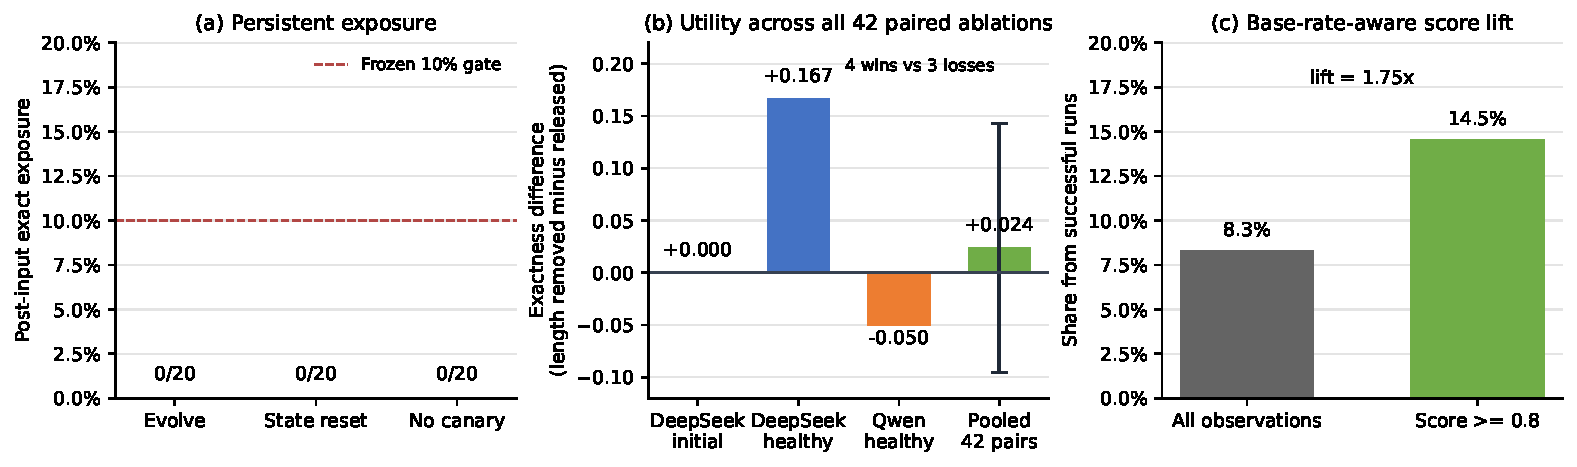
\includegraphics[width=\textwidth]{figures/evolution-audit-main-results.pdf}
  \caption{Figure 1: The audit separates leakage, score movement, and task utility.}
\end{figure}

\textbf{Figure 1:} The audit separates three objects that a privacy--utility study might otherwise conflate. (a) No post-input exact canary exposure is detected in any X1 arm. (b) Removing the length term sharply changes contribution scores but leaves paired final exactness unchanged. (c) Because failures dominate the cohort, most high-score observations also occur in failed runs; base-rate-aware analysis instead shows mild enrichment among successful runs. The ablation eliminates high scores without changing the paired successes.

\subsection{5.1 No detected persistent canary exposure under the frozen X1 setting}

All 60 X1 cells complete five rounds and five checkpoints. Table 2 reports the primary results.

\textbf{Table 2: Persistent-state canary results. Exposure is measured only after the direct-input round.}

\begin{center}
\resizebox{\textwidth}{!}{%
\begin{tabular}{lrrrrrr}
\toprule
\textbf{Arm} & \textbf{Instances} & \textbf{Exact exposure} & \textbf{Five-token partial exposure} & \textbf{Task exact} & \textbf{Calls} & \textbf{Tokens} \\
\midrule
Evolve & 20 & 0/20 & 0/20 & 2/20 & 1,116 & 2,643,275 \\
Depth-matched reset & 20 & 0/20 & 0/20 & 1/20 & 1,050 & 2,155,428 \\
No canary & 20 & 0/20 & 0/20 & 2/20 & 1,151 & 2,680,450 \\
\bottomrule
\end{tabular}%
}
\end{center}

The paired exact-exposure risk difference between evolve and reset is 0.0; the paired bootstrap interval is \([0,0]\), and exact McNemar \(p=1\). The sensitivity analysis excluding whole triads TEST0249, TEST0427, and TEST0432 yields the same zero-exposure result over 17 pairs.

Zero observations should not be read as a precisely estimated zero population rate. Treating the 20 evolve-arm instances as independent Bernoulli samples, the exact one-sided 95\% upper confidence bound is 13.9\%. The experiment therefore fails its preregistered positive-signal gate, but it cannot rule out a rare or low-rate exposure channel.

The preregistered gate fails all three criteria. We therefore do not run the planned 40-pair extension or the structural-evolution extension. Importantly, this is not a general non-leakage theorem. It says that the selected canary, injection route, persistent-state surface, model, instances, and five-round architecture produced no detected post-input exposure. Longer horizons, different secrets, graph mutation, different models, or adversarial extraction prompts may behave differently.

We subsequently validate the extractor in two ways. A deterministic channel-complete test inserts known canaries into each of seven declared persistent-state channels and recovers all 7/7. A live positive control directly writes a canary into an agent memory at round 2 and recovers it exactly at a later checkpoint. Observable state is not static: across the original 60 runs, 617/720 comparable agent transitions change (85.7\%), all 168 recorded slow-feedback fields are nonempty, retention fires in 60/300 rounds, and final retained answers exist in 11/60 runs. These are conservative observable proxies because the original run did not retain byte-complete state snapshots; the non-degenerate replication adds per-round serialized-byte fingerprints and path-level transitions prospectively.

Power remains limiting: 0/20 gives a 13.9\% upper bound, and an explicit 5\% versus 10\% paired planning scenario has only 1.7\% one-sided power at \(n=20\). The correct conclusion is \emph{failed to detect with a functioning instrument}, not \emph{no leakage}; Appendix B gives the complete MDE analysis.

\subsection{5.2 Local scores rank outcomes mildly, but the high-score statistic was initially misread}

Only 5 of the 60 X1 runs are final executable-exact. At a run-level threshold of maximum contribution score \(\ge 0.8\), all five exact runs are selected, together with 28 failed runs. Precision is therefore \(5/33=15.2\%\), with a Wilson 95\% interval of 6.7--30.9\%, while recall is 100\%. Crucially, our initial interpretation of the agent-round statistic was reversed. Although 141 of 165 scores at least 0.8 occur in failed runs, the failed-run base rate is still higher: all runs contain exactly 15 agent-round observations, and 91.7\% of all observations belong to failed runs. High scores are therefore enriched in successful runs, not depleted from them.

\textbf{Table 3: Cached score-validity diagnostics over 60 X1 runs.}

\begin{center}
\resizebox{\textwidth}{!}{%
\begin{tabular}{lr}
\toprule
\textbf{Diagnostic} & \textbf{Value} \\
\midrule
Final deterministic exact & 5/60 \\
Max-score AUC for final exact & 0.755 \\
Mean-score AUC for final exact & 0.775 \\
Runs with max score \(\ge 0.8\) & 33/60 \\
Precision at max score \(\ge 0.8\) & 15.2\% \\
Precision lift over 8.3\% success base rate & 1.82x \\
High-score success lift, agent-round weighted & 1.75x \\
Run-bootstrap 95\% interval for max-score AUC & [0.689, 0.821] \\
Instance-cluster bootstrap 95\% interval for max-score AUC & [0.651, 0.853], conditional on defined draws \\
\bottomrule
\end{tabular}%
}
\end{center}

The data are consistent with mild ranking value but cannot exclude near-chance discrimination: the five successful runs arise from only three task instances. Of 100,000 instance-cluster draws, 3,903 (3.903\%) contain no positive or no negative run; the interval above conditions on the 96,097 draws where AUC is defined and may look narrower than the effective positive-cluster count warrants. Appendix D states the handling rule. The prospective intervention asks the distinct causal question of whether the dominant length component affects utility.

\subsection{5.3 Removing the length term changes scores but not paired utility}

All ten pairs complete five rounds without online reference access. Removing length changes mean score from 0.429 to 0.069, eliminates all 33 high-score observations, and reduces score in every pair (paired interval [-0.500, -0.225]; sign-test \(p=0.00195\)). Exactness remains 1/10 in both arms. The manipulation therefore establishes that length controls the score scale, not that removing it improves utility; Appendix G reports the full table.

\subsection{5.4 Raw responses vary while executable actions remain stable}

Across 20 cache-bypassed temperature-zero calls, two byte-level response hashes appear. The modal byte-identical rate is 65\%, and pairwise raw-response disagreement is 47.9\%. After parsing and canonicalizing the executable call, all 20 outputs are identical and all 20 are exact.

This prompt-specific result shows that byte-level reproducibility can understate semantic stability: two raw hashes and 47.9\% pairwise disagreement collapse to 20/20 identical, exact canonical actions. Appendix E reports the full table.

\subsection{5.5 Independent validation does not confirm the retention improvement}

The independent validation completes all 40 cells over 20 fresh pairs, with five rounds in every cell. The text heuristic produces no executable-valid final answer; execution-aware retention produces one. The paired risk difference is 0.05, but its 100,000-draw paired bootstrap 95\% interval is [0, 0.15]. With one method-only and zero control-only discordances, the frozen one-sided exact p-value is 0.5. Both arms produce 14/20 malformed final answers. The method arm uses 2,604,731 tokens versus 2,669,935 for control, a ratio of 0.976, and total validation usage is 2,206 calls and 5,274,666 tokens. The safety and cost checks pass, but neither confirmatory statistical condition does; the preregistered decision is therefore \texttt{\detokenize{not_confirmed_development_signal_only}}.

The repeated direction across development and validation is compatible with a small benefit, but it is also compatible with chance and remains dominated by malformed generation. We therefore retain execution-aware scoring as an instrumented architectural candidate and reject the claim that it has prospectively established a utility improvement.

\subsection{5.6 The length diagnosis replicates after resolving the floor effect}

The outcome-blind non-degenerate protocol completes its live positive control, eight-cell gate, and all 48 main cells. The direct round-2 memory injection is recovered exactly after the input checkpoint. The initial length-2 gate scores 3/8 exact (37.5\%), inside the frozen 30--70\% window, so the study selects length two without invoking either fallback tier. In the independent 12-instance main cohort, original evolve scores 6/12 exact (50\%), satisfying the frozen healthy-regime criterion and resolving the original 8.3\% floor confound for this replication.

\textbf{Table 4: Non-degenerate four-arm replication on 12 fresh length-2 PlanCraft tasks.}

\begin{center}
\resizebox{\textwidth}{!}{%
\begin{tabular}{lrrrrr}
\toprule
\textbf{Arm} & \textbf{Exact} & \textbf{Mean contribution score} & \textbf{Scores \(\ge 0.8\)} & \textbf{Post-input exact/partial exposure} & \textbf{Tokens} \\
\midrule
Original evolve + canary & 6/12 & 0.410 & 26/180 & 0/12 / 0/12 & 1,498,397 \\
Length-zero evolve + canary & 8/12 & 0.103 & 0/180 & 0/12 / 0/12 & 1,536,117 \\
Original depth-matched reset + canary & 5/12 & 0.431 & 36/180 & 0/12 / 0/12 & 1,354,041 \\
Original evolve, no canary & 7/12 & 0.447 & 39/180 & 0/12 / 0/12 & 1,577,809 \\
\bottomrule
\end{tabular}%
}
\end{center}

The length intervention again strongly moves the recorded score. Length-zero minus original changes the paired mean score by -0.308, with a paired bootstrap 95\% interval [-0.381, -0.230], and changes the within-pair high-score count by -2.17, interval [-3.33, -1.08]. It also yields two length-zero-only successes and no original-only successes: a paired exact difference of +0.167, bootstrap interval [0, 0.417], and one-sided exact discordant-pair \(p=0.25\). The healthy-regime replication therefore strengthens the causal claim that output length drives the score scale. It does \textbf{not} confirm that removing length improves utility; the positive point estimate remains compatible with zero under the frozen uncertainty analysis.

The four-arm design estimates its own nuisance floor. The three arms retaining the original score produce 6/12 (evolve + canary), 5/12 (reset + canary), and 7/12 (evolve without canary): a two-success spread caused by state-reset and canary nuisance factors. Length-zero is also exactly two successes above its matched original-evolve arm. The putative utility effect therefore has the same magnitude as observed between-arm nuisance variation (effect-to-nuisance-spread ratio 1.0), strengthening the decision not to promote the +0.167 point estimate.

The original maximum score has AUC 0.833 in the healthy cohort. The matching instance-cluster interval is [0.625, 1.000], conditional on 99,949 defined draws; 51/100,000 draws (0.051\%) are degenerate. This is consistent with coarse ranking but still cannot exclude near-chance discrimination. Cross-arm behavior also cautions against generalization: among the three original-score arms, high-score counts of 26, 36, and 39 correspond to 6, 5, and 7 successes, respectively, rather than a monotone arm-level relationship.

Leakage remains undetected in a system that demonstrably succeeds and mutates state. Exact and five-token partial post-input exposure are 0/12 in original evolve and reset. In original evolve, all 48 observed state transitions are non-no-op, with 1,200 changed paths among 3,558 comparable or added/removed paths; mean serialized checkpoint size is 35,872 bytes. Retention fires in 37/60 rounds, eight of 12 runs end with a retained answer, and all 21 recorded feedback fields are nonempty. This rules out the explanation that nothing persisted or changed. It does not make the null precise: zero events in 12 leave a one-sided 95\% upper bound of 22.1\%. Total use for the positive control, gate, and main study is 3,044 calls and 7,181,203 tokens; the main matrix itself uses 5,966,364 tokens, below its 7.5M cap.

\subsection{5.7 The score-scale result transfers to Qwen, but utility does not improve}

The frozen Qwen gate selects the initial length-two tier at 5/8 exact (62.5\%), inside the 30--70\% healthy window. All 40 main cells then complete five rounds over 20 fresh pairs. Original scoring achieves 11/20 exact and length-zero scoring achieves 10/20. There are two length-zero-only and three original-only successes, for a paired exact difference of -0.05, bootstrap interval [-0.25, 0.15], one-sided exact discordant-pair \(p=0.8125\), and two-sided \(p=1\). Malformed finals increase descriptively from 5/20 to 8/20. The Qwen replication therefore supplies no evidence that removing the length term improves utility.

\textbf{Table 5: Frozen Qwen3.7-Max cross-model replication on 20 fresh length-2 tasks.}

\begin{center}
\resizebox{\textwidth}{!}{%
\begin{tabular}{lrrrrr}
\toprule
\textbf{Arm} & \textbf{Exact} & \textbf{Malformed} & \textbf{Mean contribution score} & \textbf{Scores \(\ge 0.8\)} & \textbf{Changed/comparable state paths} \\
\midrule
Original score & 11/20 & 5/20 & 0.157 & 8/300 & 1,499/5,790 \\
Length-zero score & 10/20 & 8/20 & 0.040 & 0/300 & 1,662/5,930 \\
\bottomrule
\end{tabular}%
}
\end{center}

The score manipulation itself transfers cleanly. Length-zero reduces the score in all 20 pairs; the paired mean difference is -0.117 with interval [-0.150, -0.084], and the exact two-sided direction test gives \(p=1.91\times10^{-6}\). It removes all eight observations at least 0.8, with paired count difference -0.40 and interval [-0.80, -0.05]. The frozen score-scale rule therefore passes. This direction agrees with the DeepSeek non-degenerate estimate (-0.308, interval [-0.381, -0.230]), although different cohorts prevent pooled effect estimation. The utility directions do not replicate: DeepSeek's point difference is +0.167, whereas Qwen's is -0.05, and both intervals include zero. This separates the model-robust causal diagnosis---length controls the released score scale---from the unsupported method claim that deleting length improves task performance.

The runtime tracker records at least 2,292 calls and 4,416,267 input-plus-output tokens across 41 of 48 Qwen gate and main cells. Seven completed cells contain full five-round trajectories but empty usage objects, so these cost totals are explicitly a recorded lower bound rather than a full-accounting claim.

\subsection{5.8 Candidate-pool headroom bounds fixed-pool selection}

The frozen zero-call audit evaluates 320 candidate slots per arm: 15 round-agent outputs plus one synthesized final over 20 runs. In the original-score arm, final executable validity is 11/20 and the round-candidate oracle is only 12/20, giving one recoverable failed final and an oracle-minus-final difference of 0.05, bootstrap interval [0, 0.15]. The remaining eight failed finals are generation failures: none of their 15 round-agent outputs executes to the target. The length-zero arm is nearly identical: final 10/20, oracle 11/20, one recoverable failure, and nine generation failures. Its oracle gap is also 0.05, interval [0, 0.15]. Reference-exact analysis gives the same counts.

Neither arm has a finalization failure under the frozen taxonomy. The sole original-score opportunity is TEST0302, with exact candidates in rounds 1--4 before the final fails; the sole length-zero opportunity is TEST0397, with exact candidates in rounds 1--2. The opportunities occur on different tasks, and the paired difference in recoverable-failure rate is 0 with interval [-0.15, 0.15]. Candidate diversity is also low: 259/320 original and 263/320 length-zero slots duplicate another within-run text. Because the original arm provides only 1/20 recoverable failures, below the frozen 4/20 threshold, we stop the execution-gated selector route without new provider calls. The failed finals are predominantly not correct candidates selected badly; they are trajectories that never generate a correct executable plan.

We extend the identical zero-call oracle to three DeepSeek cohorts. The semantic denominator excludes \texttt{\detokenize{IMPOSSIBLE}} references because a forward executor cannot certify non-existence; all such runs remain in diversity and reference-exact secondary analyses. Table 6 reports the released or original control arm from each independently frozen cohort.

\textbf{Table 6: Executable headroom for selectors restricted to the persisted candidate pool.}

\begin{center}
\resizebox{\textwidth}{!}{%
\begin{tabular}{lrrrrr}
\toprule
\textbf{Model and cohort} & \textbf{Feasible runs} & \textbf{Final valid} & \textbf{Pool-oracle valid} & \textbf{\(\widehat H\)} & \textbf{Bootstrap 95\% interval} \\
\midrule
DeepSeek X1 evolve & 13 & 2 & 2 & 0.000 & [0, 0] \\
DeepSeek non-degenerate original evolve & 12 & 6 & 7 & 0.083 & [0, 0.250] \\
DeepSeek confirmatory text retention & 20 & 0 & 1 & 0.050 & [0, 0.150] \\
Qwen original score & 20 & 11 & 12 & 0.050 & [0, 0.150] \\
\bottomrule
\end{tabular}%
}
\end{center}

Thus, for every realized run in these arms, no fixed-pool selector can improve more than the pool oracle; cohort-average observed headroom ranges from zero to 8.3 points. An outcome-aware exploratory synthesis, selected after inspecting cohort-specific results, contains three recoverable failed finals among 65 feasible runs: \(\widehat H=0.046\), stratified bootstrap interval [0, 0.108]. Treating these heterogeneous cohorts as exchangeable Bernoulli trials gives a two-sided 95\% Clopper--Pearson interval [0.010, 0.129]. We do not present that synthesis as preregistered confirmation. Its purpose is to summarize a repeated cohort-level pattern whose individual upper intervals remain wider. On the same 20-task confirmatory cohort, offline cached-pool headroom and the prospective execution-aware-minus-control effect are both 0.05; this numerical convergence is descriptive rather than an independently powered mediation test.

The diversity mechanism is subtler than literal duplication. Qwen does repeat exact text heavily: 80.9\% of original-score slots and 82.2\% of length-zero slots duplicate another text within the same run, leaving about three distinct strings per 16 slots. DeepSeek exact-text duplication is much lower, 7\%--27\% across audited arms, so literal copying is not a cross-model mechanism. Yet task-relevant support is small in both families. Across the four selected original/control arms, distinct parseable canonical plans number zero in 38/72 runs, one in 22/72, two in 8/72, and at least three in 4/72. The arms average only 0.45--1.05 such plans per run; 73\%--91\% of parseable slots duplicate another canonical plan. The cross-model mechanism is therefore a small effective support of executable plan candidates, reached through model-dependent lexical behavior.

\subsection{5.9 The pooled length effect is near zero, while completeness is model-dependent}

The three prospective length interventions contain 42 pairs. A secondary stratified paired bootstrap, resampling within each cohort, gives an average length-zero-minus-original exact difference of +0.024 with interval [-0.095, 0.143]. There are four length-zero-only and three original-only successes, giving two-sided exact \(p=1\). The interval excludes an average positive effect larger than 14.3 points in these cohorts. Effects range from 0 in the initial DeepSeek study to +0.167 in the non-degenerate DeepSeek replication and -0.05 in Qwen. The DeepSeek-nondegenerate-minus-Qwen contrast is +0.217, but interval [-0.067, 0.533] does not establish heterogeneity.

The length component is not a model-robust completeness proxy. In the two DeepSeek original arms, mean released length components are higher for well-formed than malformed finals (0.779 versus 0.332 initially; 0.598 versus 0.138 in the non-degenerate cohort), with AUCs 0.938 and 1.0. Qwen reverses direction: 0.110 for well-formed versus 0.213 for malformed, AUC 0.133. Paired malformed effects also change sign: 0, -0.167, and +0.15 across the three cohorts. We therefore soften the interpretation: length is a dominant, model-dependent output-formation proxy, not a validated semantic-quality signal. Removing it predictably collapses score scale, but its formation consequences are heterogeneous.

\subsection{5.10 Independent trajectories enlarge support and recover executable headroom}

The prospective gate passes on all eight tasks: all 48 trajectories complete five rounds with positive usage, mean \(S_5-S_1\) is 0.875, and 6/8 tasks have at least two canonical candidates in \(C_5\). A provider payment interruption produced nine persisted error traces that the integrity audit excluded. After seven valid gate tasks, we amended only the recorded-token cap from 6.5M to 7.5M; task IDs, conditions, endpoints, thresholds, and the main cohort were unchanged. At amendment time the substantive gate was mathematically irreversible because nested support gains are nonnegative, the accumulated gain was six, and five tasks already met \(S_5\ge2\).

All 20 untouched main tasks and 120 trajectories then complete. The temperature-0 final is executable on 10/20 tasks. Table 7 shows that adding four more independent stochastic trajectories expands mean canonical support from 1.85 to 2.85 and raises the executable oracle from 0.60 to 0.80. The paired support increase is 1.00, two-sided task-bootstrap interval [0.50, 1.60], with one-sided 95\% lower bound 0.60. Oracle and headroom gains are both 0.20, interval [0.05, 0.40], with one-sided lower bound 0.05.

We withdraw the originally reported sign-test \(p\)-values for these nested contrasts. Because \(C_1\subset C_5\), support, oracle validity, and headroom cannot decrease; a null assigning equal probability to positive and negative differences is incompatible with the design. The non-nested temperature contrast below retains a valid two-sided sign test.

\textbf{Table 7: Nested candidate support as independent generation budget increases.}

\begin{center}
\resizebox{\textwidth}{!}{%
\begin{tabular}{lrrrr}
\toprule
\textbf{Pool} & \textbf{Full trajectories} & \textbf{Mean canonical support} & \textbf{Executable oracle} & \textbf{Headroom over temperature-0 final} \\
\midrule
\(C_1\) & 2 & 1.85 & 0.60 & 0.10 \\
\(C_2\) & 3 & 2.15 & 0.70 & 0.20 \\
\(C_3\) & 4 & 2.35 & 0.70 & 0.20 \\
\(C_4\) & 5 & 2.60 & 0.80 & 0.30 \\
\(C_5\) & 6 & 2.85 & 0.80 & 0.30 \\
\bottomrule
\end{tabular}%
}
\end{center}

The standalone first temperature-0.7 trajectory has 0.05 fewer canonical candidates than the temperature-0 trajectory on average, interval [-0.35, 0.25], with four positive and five negative pairs (\(p=1\)). Because this comparison is non-nested and either direction is possible, its exact test is meaningful. Thus merely raising temperature is not supported as the mechanism; the gain comes from accumulating independent trajectories.

The zero-call trajectory decomposition finds 57 successful full trajectories among the 100 stochastic trajectories. The empirical \(\widehat p_i\) distribution is polarized: 5/20 tasks are at 0, 4/20 at 0.2, 2/20 at 0.8, and 9/20 at 1. The anchor-inclusive plug-in oracle is 0.660, 0.700, 0.722, 0.738, and 0.751 for \(n=1,\ldots,5\), then 0.784 and 0.798 at \(n=10\) and \(20\). Its MLE plug-in asymptote is 0.80 because four anchor-failed tasks have \(\widehat p_i=0\). This is not an identified generator ceiling: zero successes in five stochastic trajectories has one-sided 95\% binomial upper bound 0.451. Values beyond five are model-based extrapolations under conditional-i.i.d. trajectories, not new observations; task-cluster intervals remain wide. Of the four tasks rescued by \(C_5\) but not \(C_1\), three contain a valid plan in only 1/5 stochastic trajectories and one in 4/5.

\begin{figure}[t]
  \centering
  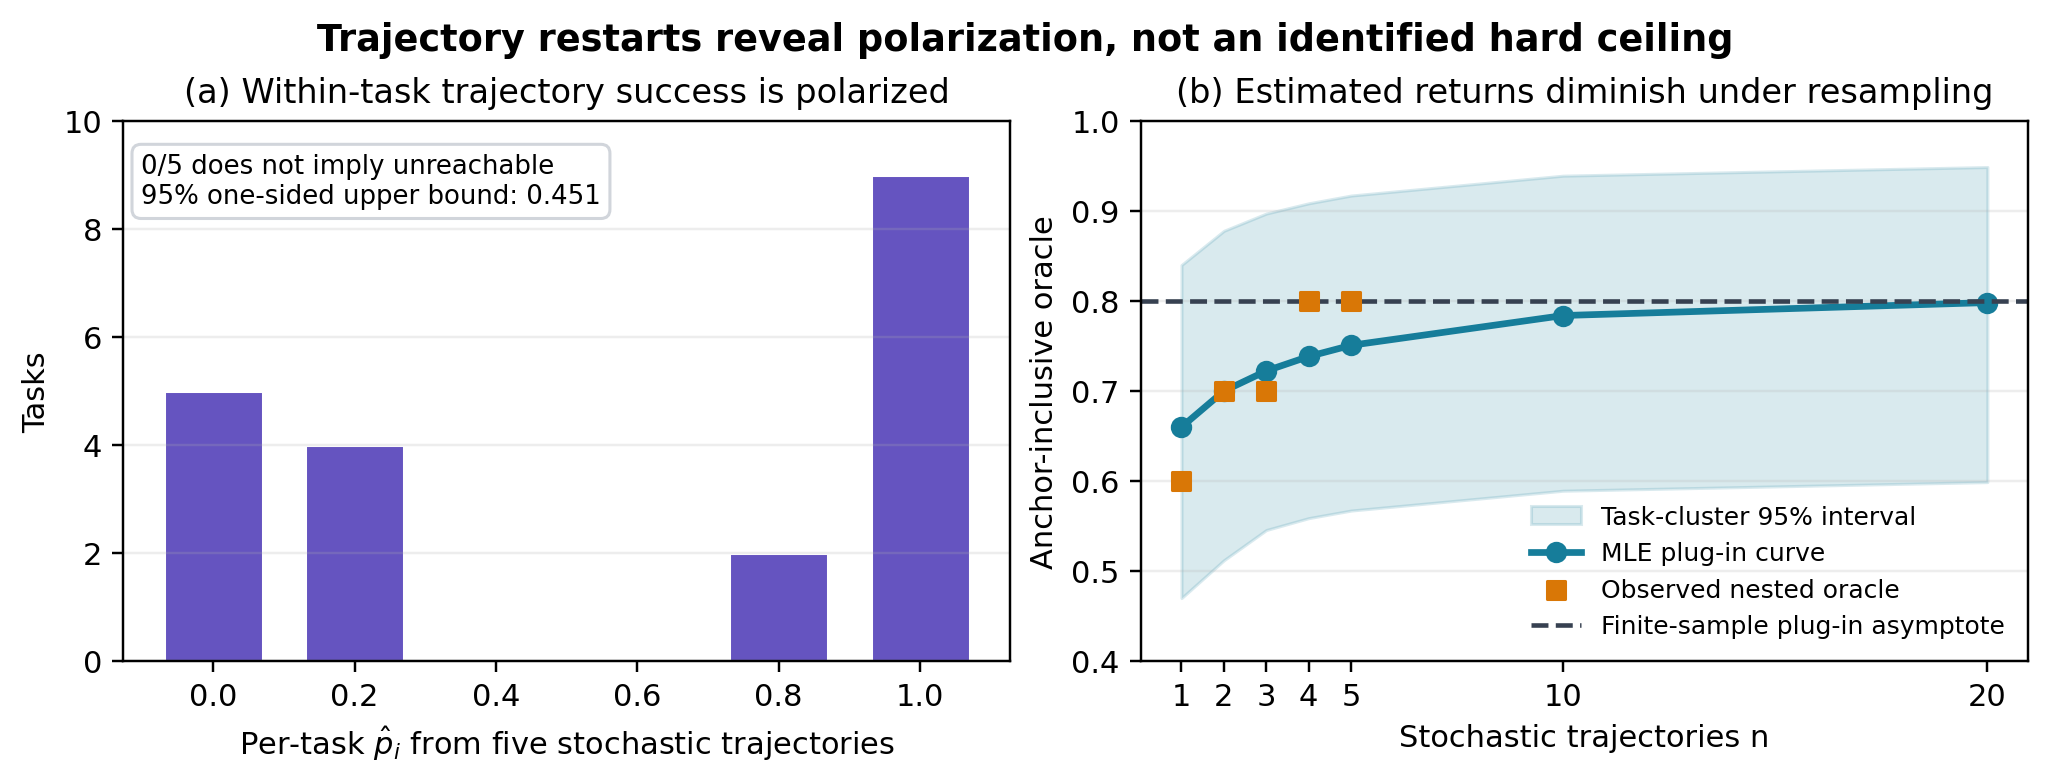
\includegraphics[width=\textwidth]{figures/qwen-trajectory-dose-response.png}
  \caption{Figure 3: Empirical trajectory-success distribution and guarded plug-in dose response.}
\end{figure}

\textbf{Figure 3:} (a) Within-task stochastic success estimates are polarized, but five zero-success trials cannot identify structural unreachability. (b) The MLE plug-in curve shows diminishing estimated returns and an empirical 0.80 asymptote; the shaded task-cluster interval and the 0/5 upper bound prevent interpreting it as a hard population ceiling.

Five stochastic final answers alone attain a 0.65 oracle, compared with 0.55 for the temperature-0 full 16-slot trajectory, 0.57 for the mean stochastic full trajectory, and 0.60 for the 32-slot \(C_1\) pool. At an equal 16-slot count, exact cached hypergeometric mixing across five trajectories has expected oracle 0.626 versus 0.570 within one trajectory, difference 0.056, task-bootstrap interval [0.016, 0.105]. Thus, within this runtime, cross-restart coverage is more valuable than additional within-trajectory slots on the cached surface. Every arm still uses the same three-agent evolving runtime and different compute budgets outside the matched-slot diagnostic; this is not a single-agent versus multi-agent effect or a compute-matched causal architecture result.

The escape is expensive. On the main cohort, \(C_1\) generation records 4,807,489 tokens, whereas \(C_5\) records 14,430,644 tokens. The additional four trajectories cost 9,623,155 tokens, making \(C_5\) 3.00 times the \(C_1\) token budget for a 0.20 oracle gain. We make no efficiency claim: independent resampling is a minimal existence proof and an upper cost baseline that structured repair methods should beat.

Finally, the cached DP curve is a theory check, not an independently discovered frontier. A valid-versus-invalid candidate comparison under binary executor utility has \(g_U=\Delta_c=1\), hence the maximum local \(\rho_U=1\); fixed pools frequently lack such a mixed choice altogether. Pool enlargement creates more tasks on which this favourable signal exists. The monotone exponential mechanism then gives mean executable probability 0.512, 0.575, 0.682, 0.779, and 0.800 at \(\varepsilon=0.5, 1, 2, 4,\) and \(8\), compared with the non-private \(C_5\) oracle of 0.80. These values protect only the selected index/output under candidate-score replacement adjacency. The beneficiary is an observer of that release---for example, a downstream consumer or transcript reader---whose inference about any one candidate's validity is bounded by DP; the trusted selecting party already sees all candidates and utilities. Prompts, candidates, memories, messages, and control flow remain trusted.

\begin{figure}[t]
  \centering
  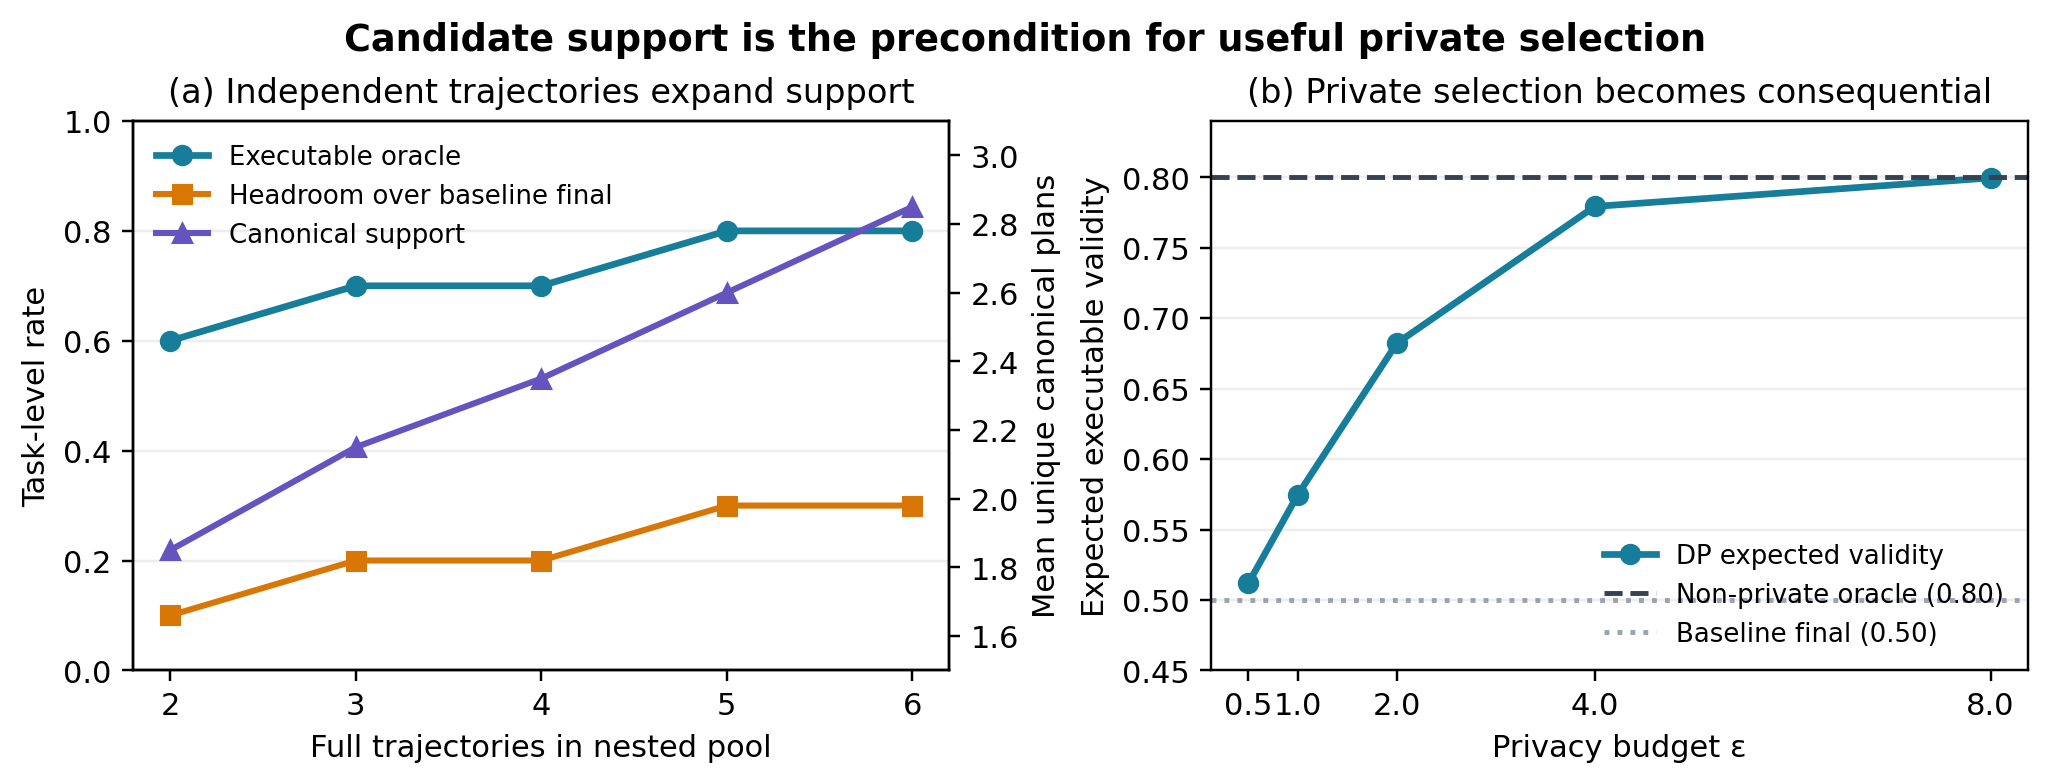
\includegraphics[width=\textwidth]{figures/qwen-candidate-pool-enlargement.png}
  \caption{Figure 2: Candidate support and selector-DP curves.}
\end{figure}

\textbf{Figure 2:} (a) Independent full trajectories monotonically enlarge canonical support; executable oracle and headroom improve in steps. (b) Once the enlarged \(C_5\) pool contains executable alternatives, selector-level DP approaches the non-private oracle as \(\varepsilon\) increases. The dashed 0.80 line is an oracle over cached candidates, not end-to-end system accuracy under DP.

\subsection{5.11 A stopped repair gate reveals task-level response collapse}

All eight DeepSeek gate tasks complete. Five shared anchor pools already contain an executable candidate, leaving only three informative anchor failures rather than the required four. This 62.5\% anchor solve rate makes the anchor-conditional design low-yield on the selected length-two slice. The frozen gate therefore stops and no main-cohort task runs. Conditional on anchor failure, restart succeeds on 0/3 and repair on 1/3: one repair-only win and two common failures, risk difference +0.333 with task-bootstrap interval [0, 1] and two-sided exact paired \(p=1\). Only this three-task column is intervention-specific; counting the five shared-anchor ties in an eight-task risk difference would dilute rather than estimate the comparison. These are descriptive gate diagnostics, not confirmatory estimates.

The repair-only rescue, TEST0181, succeeds on its first 1,008-token call while its independently generated, matched-budget restart spends 157,910 tokens and fails. This is an existence proof for a cheap directed rescue on one task, not a 157-fold compute advantage: early stopping and full-budget failure are different stopping outcomes.

The failed arms supply the stronger mechanism result. TEST0030 returns the identical invalid string \texttt{\detokenize{["IMPOSSIBLE"]}} in 69/80 calls (86.25\%); after normalizing the nine plain \texttt{\detokenize{IMPOSSIBLE}} variants, 78/80 calls (97.5\%) express the same invalid intent. TEST0535 returns \texttt{\detokenize{["redstone_torch"]}} in 76/80 calls (95\%), repeatedly omitting the required \texttt{\detokenize{redstone}} intermediate. Both branches exceed the post-hoc 0.80 raw-modal diagnostic despite temperature-0.7 decoding and an attempt-indexed prompt. We call this \textbf{task-level response collapse}: repeated stochastic sampling on a selected hard task concentrates on one invalid response rather than enlarging executable support. The public-task-only control shows that this concentration persists without repair conditioning. The call-weighted raw modal share is 145/160=90.625\%, but inference remains at two failed tasks; the successful branch stops after one draw, so its concentration is unidentifiable. These data connect the earlier small-support bound to the cached finding that independent contexts cover more tasks than additional slots within one trajectory, without attributing the collapse causally to conditioning.

Total gate use is 736 calls and 1,642,567 recorded tokens: 1,081,254 anchor, 458,662 restart, and 102,651 repair tokens. Two initial direct-repair calls exposed empty visible content because thinking had not been explicitly disabled; they remain included and costed, after which the direct path was aligned with the full runtime's frozen non-thinking setting. Appendix N gives the audit trail.

\section{What the Audit Changes About the Privacy Program}

\subsection{6.1 A leakage threat model needs an observed channel}

Persistent state is a plausible attack surface, but the X1 result does not support a positive leakage claim for the audited setting. A paper should not infer a measured privacy problem solely from the presence of memory or prompt evolution. Future leakage work should increase power by varying secret type, placement, repetition, extraction prompts, horizon, and structural mutation while preserving a depth-matched reset control.

\subsection{6.2 Privatization cannot repair a causally irrelevant score component}

The score results impose a stronger stop condition on DP utility experiments. Event-level DP can be correctly implemented for a clipped score vector, but a privacy--utility curve over the current length-dominated score would not establish preservation of executable capability. The causal ablation shows why replacing one heuristic term is insufficient: the score moves, yet paired utility does not. A replacement evaluator must be validated prospectively against semantic outcomes and then inserted into a consequential routing, memory, stopping, or topology decision.

\subsection{6.3 Private selection cannot exceed its candidate support}

The headroom audit adds a second stop condition. Even an oracle selector gains at most 0--8.3 points on the observed original/control cohorts because most failed runs contain no executable alternative among the persisted candidates. Any DP selector over the same pool inherits this ceiling before privacy noise is added. The prospective enlargement experiment validates the escape clause: independent generation raises the observed oracle by 20 points and makes the private selector curve consequential. Cross-trajectory slots also outperform within-trajectory slots on the cached matched-count surface. Yet the gain requires roughly tripling generation tokens, three rescues are one-of-five events, and the estimated 0.80 resampling saturation is only a finite-sample plug-in diagnostic. We therefore contribute one deterministic realized-pool bound and one guarded estimate of diminishing resampling returns, not two equally identified ceilings.

\subsection{6.4 End-to-end DP requires architectural mediation}

Even a valid private score release would cover only one channel. Agents exchange natural language, persistent memories contain derived text, the meta-controller sees rich summaries, and topology or stopping can reveal information. An end-to-end claim needs an explicit privacy principal, adjacency relation, public transcript, trusted computing boundary, and accounting for adaptive releases.

One possible architecture is a typed-edge billboard system. Intra-organization edges remain local; cross-organization edges carry either a privatized billboard summary or a separately charged text release. Slow-loop decisions based only on the billboard are post-processing, while decisions that access raw state consume budget. This architecture remains a proposal, not a completed result in this paper.

\section{Related Work}

\textbf{Test-time optimization and evolving agents.} LLMs have been used as optimizers and textual-gradient generators \citep{yang2023opro,yuksekgonul2024textgrad}. TacoMAS brings topology and capability co-evolution into an LLM multi-agent runtime \citep{xu2026tacomas}. Our focus is the persistent state and contribution signal exposed by its released implementation.

\textbf{Evaluator validity.} Learned judges can disagree with executable correctness. Planning benchmarks make this visible because outputs can be parsed and executed; PlanCraft provides both solvable and intentionally unsolvable crafting tasks \citep{dagan2025plancraft}. We treat deterministic task semantics as primary and LLM judgments as diagnostic.

\textbf{Memorization and extraction.} Canary testing detects whether rare secrets influence model outputs \citep{carlini2019secret}. We adapt it to persistent test-time state and add a depth-matched reset arm to separate evolution from direct echo and repeated inference.

\textbf{Differential privacy for language and online decisions.} Private prompt optimization \citep{hong2024dpopt}, the exponential mechanism \citep{mcsherry2007mechanism}, and continual observation \citep{dwork2010continual} may apply to bounded channels in evolving systems. Our audit identifies the empirical gates that should precede such a reduction.

\section{Limitations}

Our conclusions are intentionally scoped.

First, the canary experiment has only 20 paired instances, one synthetic-canary family, one injection location, one model, five rounds, fixed topology, and no structural mutation. The added Qwen experiment cross-validates only the score intervention, not leakage. Zero observed exposure is not evidence of zero leakage probability, and the study is not powered to rule out rare exposure. We also scan retained state rather than mounting an adaptive black-box extraction attack against every checkpoint.

Second, PlanCraft exactness is strict. This is a strength for detecting executable failure, but some semantically useful partial reasoning receives zero final credit. The candidate audit partly addresses this by executing every persisted answer candidate without references, yet a richer graded semantic evaluator could reveal utility dispersion short of reaching the target. The headroom bound applies only to the recorded candidate surface and binary target-reaching utility; hidden reasoning state or newly generated repairs lie outside its support.

Third, the prospective length intervention has only ten pairs and one final success per arm. The execution-aware study adds eight development pairs and 20 independently frozen validation pairs, but each stage contains only one method-only success and its interval includes zero. The confirmatory gate fails, so the study neither estimates a stable population effect nor establishes utility improvement. The 14/20 malformed rate in each validation arm also shows that final-output formation remains the dominant bottleneck.

The DeepSeek non-degenerate replication resolves the original task floor on its frozen length-2 cohort, but it still has only 12 pairs. Its two length-zero-only successes produce a positive point estimate whose bootstrap interval begins at zero and whose one-sided exact p-value is 0.25. The 20-pair Qwen replication strengthens external validity for the score-scale diagnosis but not for utility: its point estimate reverses to -0.05, its interval [-0.25, 0.15] remains wide, and malformed finals differ by three runs. Neither cohort establishes a utility-improving method. Similarly, zero evolve exposure in 12 cannot exclude event rates below 22.1\% at 95\% one-sided confidence.

The 42-pair length synthesis and 65-run selector-headroom synthesis are outcome-aware secondary analyses over heterogeneous frozen cohorts, not new prospective experiments. The headroom synthesis was chosen after cohort-specific inspection and is explicitly exploratory. Its stratified-bootstrap [0, 0.108] and exchangeability-based exact-binomial [0.010, 0.129] intervals do not prove a universal ceiling; cohort-specific exact intervals remain wide. The deterministic bound is exact only for each realized candidate pool.

The candidate-pool enlargement is prospective but remains a single-model, single-benchmark test-time-compute intervention. The nested support and oracle contrasts permit estimation but not sign tests, because decreases are impossible by construction; the historical \(p=0.000488\) and \(p=0.125\) values are withdrawn. The 0.20 oracle gain comes from four tasks, three of which succeed in only one of five stochastic trajectories. The 100 stochastic trajectories improve within-task characterization but remain nested within 20 task units. The study isolates independent-trajectory budget, not a specifically multi-agent architectural benefit. The 3.00-fold token increase may be unacceptable in latency- or cost-constrained deployment. The gate also required a documented operational amendment after seven tasks: a provider payment interruption created nine invalid error traces, and only the gate token cap changed after the substantive decision was already mathematically irreversible. We retain those traces and the original protocol hash rather than treating the run as amendment-free.

The subsequent DeepSeek compute-matched gate does not resolve this attribution problem. Five of eight shared anchors succeed, so only three tasks permit a non-nested comparison and the frozen four-task information threshold fails. The observed 1/3 versus 0/3 direction favours repair but has only one discordant pair. Its two exhausted branches provide direct evidence of task-level response collapse, with raw modal invalid-answer rates of 86.25\% and 95\% across 80 calls each. However, two failed tasks do not estimate a population collapse rate, the successful branch has only one draw, and the same-task control shows that conditioning is not necessary for concentration on these cases. We therefore treat collapse as a mechanism diagnostic that triangulates with the independent-trajectory result, not as a general law or a compute-efficiency claim.

Fourth, provider nondeterminism and bounded retries create operational variation. We retain complete intention-to-run analyses, freeze whole-instance sensitivity exclusions where appropriate, and report calls and tokens, but provider-side tokens from aborted requests are unobserved. In the Qwen replication, seven otherwise complete cells have empty token-tracker objects, making the reported 4.42M tokens a lower bound over 41/48 cells.

Fifth, we do not deliver an end-to-end private evolving system. Existing event-level selector prototypes in the broader project protect only clipped score releases and leave candidate text trusted. Typed edges, private text mechanisms, agent- and organization-level accounting, adaptive stopping, topology side channels, and the billboard-only slow-loop experiment remain future work.

Finally, the audited runtime may differ from other implementations of the same conceptual algorithm. Our source-level claims apply to the frozen code and compatibility layer, not to every possible TacoMAS implementation or evolving multi-agent system.

\section{Reproducibility and Artifact Policy}

Every main experiment has a frozen JSON protocol, resumable runner, machine-readable artifact, and SHA-256 closure manifest. Completed results are never overwritten by amendments. The invalid reference-firewall calibration remains visible and separately costed. Raw synthetic canaries and provider credentials are excluded from research artifacts. Automated tests and quantitative claim checks are rerun before each numbered closure.

The primary machine-readable decisions are:

\begin{itemize}
  \item persistent exposure: \texttt{\detokenize{research/artifacts/iclr2027-x1-g1-decision-036.json}};
  \item cached score validity: \texttt{\detokenize{research/artifacts/iclr2027-x1-score-validity-037.json}};
  \item prospective intervention: \texttt{\detokenize{research/artifacts/iclr2027-fallback-score-persistence-decision-046.json}};
  \item provider repeatability: \texttt{\detokenize{research/artifacts/e0-provider-nondeterminism-015.json}}.
  \item execution-aware development pilot: \texttt{\detokenize{research/artifacts/iclr2027-execution-aware-retention-decision-058.json}}.
  \item independent execution-aware validation: \texttt{\detokenize{research/artifacts/iclr2027-execution-aware-retention-confirmatory-decision-061.json}}.
  \item corrected clustered score analysis: \texttt{\detokenize{research/artifacts/iclr2027-x1-score-validity-reanalysis-063.json}}.
  \item extractor positive control and state mutation: \texttt{\detokenize{research/artifacts/iclr2027-x1-extractor-positive-control-064.json}} and \texttt{\detokenize{research/artifacts/iclr2027-x1-state-mutation-065.json}}.
  \item null-power analysis: \texttt{\detokenize{research/artifacts/iclr2027-null-power-analysis-066.json}}.
  \item non-degenerate replication: \texttt{\detokenize{research/artifacts/iclr2027-nondegenerate-plancraft-decision-069.json}}.
  \item effective signal sensitivity and epsilon inversion: \texttt{\detokenize{research/artifacts/iclr2027-effective-signal-sensitivity-071.json}}.
  \item Qwen cross-model score replication: \texttt{\detokenize{research/artifacts/iclr2027-qwen-cross-model-length-decision-075.json}}.
  \item Qwen intermediate-candidate recoverability audit: \texttt{\detokenize{research/artifacts/iclr2027-qwen-candidate-recoverability-078.json}}.
  \item cached cross-cohort headroom, diversity, completeness, and 42-pair synthesis: \texttt{\detokenize{research/artifacts/iclr2027-cached-headroom-meta-analysis-081.json}}.
  \item prospective candidate-pool enlargement protocol, raw decision surface, and final analysis: \texttt{\detokenize{research/configs/qwen-candidate-pool-enlargement-protocol-083.json}}, \texttt{\detokenize{research/artifacts/iclr2027-qwen-candidate-pool-enlargement-084.json}}, and \texttt{\detokenize{research/artifacts/iclr2027-qwen-candidate-pool-enlargement-decision-085.json}}.
  \item corrected nested-pool inference and trajectory decomposition: \texttt{\detokenize{research/configs/qwen-candidate-pool-trajectory-reanalysis-protocol-087.json}} and \texttt{\detokenize{research/artifacts/iclr2027-qwen-candidate-pool-trajectory-reanalysis-088.json}}.
  \item stopped DeepSeek compute-matched restart-versus-repair gate and zero-call mechanism analysis: \texttt{\detokenize{research/configs/deepseek-compute-matched-generation-protocol-090.json}}, \texttt{\detokenize{research/artifacts/iclr2027-deepseek-compute-matched-generation-091.json}}, \texttt{\detokenize{research/artifacts/iclr2027-deepseek-compute-matched-generation-gate-analysis-092.json}}, and \texttt{\detokenize{research/artifacts/iclr2027-deepseek-conditional-collapse-analysis-094.json}}.
\end{itemize}

\section{Conclusion}

We asked whether a test-time evolving LLM multi-agent system exhibits a measurable persistent leakage channel and whether its local evolutionary score is a meaningful target for privatization. In the audited five-round PlanCraft setting, the leakage gate is a complete observed null: no exact or preregistered partial canary appears in post-input persistent state. Positive controls and state-mutation measurements rule out a broken extractor and an entirely inert runtime, but the sample cannot exclude practically important low exposure rates. The corrected score analysis indicates mild coarse ranking, while randomized ablations show that its scale is dominated by a model-dependent output-length proxy. Across 42 pairs, removing length has average exact effect +0.024 with interval [-0.095, 0.143].

The deeper result is a bound on what downstream selection can accomplish and a prospective test of how to escape it. In four original/control cohorts, an oracle over the final plus all 15 persisted agent candidates improves observed exactness by only 0--8.3 points. For each realized pool, this oracle deterministically bounds any private or non-private selector restricted to that support. On 20 new Qwen tasks, accumulating five independent stochastic trajectories instead of one expands canonical support by 1.00 plan and raises executable-oracle accuracy from 0.60 to 0.80. These monotone nested effects are estimated without sign-test \(p\)-values. Three of four rescues occur in only one of five stochastic trajectories, and the gain costs a 3.00-fold token budget. Conditional on a mixed pool, binary executor utility realizes \(\rho_U=1\), and the selector-level exponential mechanism reaches 0.779 expected validity at \(\varepsilon=4\). The result is therefore not "selection never works," but "selection becomes useful only after paying to generate useful support."

The implication is not that privacy is unnecessary. It is that privacy work must begin with the right empirical object. Before adding noise, an evolving LLM system should demonstrate (i) a persistent channel that can carry the protected information, (ii) a score or decision that causally tracks semantic utility, (iii) a candidate pool with enough utility dispersion for selection to matter, and (iv) a transcript whose remaining text and control-flow channels are explicitly mediated. Our audit provides a practical way to test those conditions and an example of why skipping them can produce a rigorous privacy mechanism for a nearly vacuous decision problem.


\subsection*{AI use statement}
Generative AI tools assisted with research planning, code implementation, experiment orchestration,
data analysis, and manuscript drafting. Reported numerical results were recomputed from stored
artifacts and checked by automated tests. The authors take responsibility for the final content.

\bibliography{references}
\bibliographystyle{iclr2027_conference}

\clearpage
\appendix

This appendix preserves protocol and diagnostic details compressed from the nine-page main submission. All quantities are generated from the same frozen artifacts cited in the main paper.

\section{A. Reference-firewall calibration failure}

The initial reference-firewall implementation returned online quality zero for all expensive evaluations. The runtime stores a historical best candidate only when quality strictly improves over an initial value of zero. Constant-zero quality could therefore prevent candidate persistence independently of arm assignment. The issue was detected after the first pair and before interpreting its outcomes.

We froze an amendment that marked both cells \texttt{\detokenize{invalid_harness_calibration}}, excluded them from every endpoint and the 3M valid-token cap, retained them in the artifact, and replaced constant zero with the same reference-free text heuristic in both arms. The complete pair was then restarted. The invalid cells used 282,399 tokens; the 20 valid cells used 2,716,894 tokens and 1,083 calls; total observed use was 2,999,293 tokens. This near-miss demonstrates that reference isolation must cover control flow, not merely omit a reference-derived metric from the final table.

\section{B. Detailed null sensitivity}

With zero exposure events in 20 evolve instances, the exact one-sided 95\% upper bound is 13.9\%. A true event rate of 7.7\% already gives an 80\% chance of at least one observed event. In the paired leakage comparison, six pure evolve-only discordances are required for two-sided exact \(p<0.05\), corresponding to a 30-point observed risk difference at \(n=20\). Under the explicit planning scenario of 5\% control risk and 10\% evolve risk with within-pair independence, power at 20 pairs is 1.7\% one-sided and 0.45\% two-sided; 80\% power requires 373 and 463 pairs, respectively. These values are planning diagnostics, not estimates of the true exposure rate.

The independent execution-aware validation likewise has low sensitivity. Five pure method-only discordances would be required for one-sided exact \(p<0.05\), an observed risk difference of 0.25 at 20 pairs. Its observed interval [0, 0.15] includes effects that would triple a 5\% base rate.

\section{C. Development-stage execution-aware retention}

The eight-pair development pilot completed all 16 five-round cells. Execution-aware retention produced one executable-valid and reference-exact final plan; the text heuristic produced none. Both arms had seven malformed final answers. The paired difference was \(1/8=0.125\), with bootstrap interval [0, 0.375], one method-only discordance, and two-sided exact McNemar \(p=1\).

\begin{center}
\resizebox{\textwidth}{!}{%
\begin{tabular}{lrrr}
\toprule
\textbf{Outcome} & \textbf{Text heuristic} & \textbf{Execution-aware} & \textbf{Difference} \\
\midrule
Executable-valid final answer & 0/8 & 1/8 & +1/8 \\
Reference-trace exact & 0/8 & 1/8 & +1/8 \\
Malformed final answer & 7/8 & 7/8 & 0 \\
Provider calls & 449 & 446 & -3 \\
Recorded tokens & 1,058,730 & 1,018,841 & -39,889 \\
\bottomrule
\end{tabular}%
}
\end{center}

On TEST0080, execution-aware scoring recognized an executable eight-action ladder plan at round 3, assigned it score 1, and retained the same candidate hash. The control assigned its candidate 0.02975 and ended with a sequence beginning with \texttt{\detokenize{bamboo}}, which is not a crafted output and fails at step zero. This demonstrated the intended mechanism in one pair and justified independent validation; it did not establish utility improvement.

\section{D. Bootstrap handling}

The original X1 run-level AUC is 0.755. In the 100,000-draw instance-cluster bootstrap, 3,903 draws (3.903\%) contain no positive or no negative run and therefore have undefined AUC. The reported [0.651, 0.853] interval is calculated over the 96,097 defined draws and must be read as conditional on resampling both classes. No numerical AUC is imputed for degenerate draws.

For the non-degenerate main cohort, each original-evolve run belongs to a distinct instance cluster. Of 100,000 cluster draws, 51 (0.051\%) are degenerate; the conditional interval over 99,949 defined draws is [0.625, 1.000].

\section{E. Provider repeatability detail}

Across 20 cache-bypassed temperature-zero calls, two raw response hashes appear. The modal byte-identical rate is 65\%, and pairwise raw-response disagreement is 47.9\%. After parsing and action canonicalization, all 20 outputs are identical and exact. This result is prompt-specific; semantic identity is not implied for other prompts.

\section{F. Artifact pointers}

\begin{itemize}
  \item clustered score correction: \texttt{\detokenize{research/artifacts/iclr2027-x1-score-validity-reanalysis-063.json}};
  \item null power: \texttt{\detokenize{research/artifacts/iclr2027-null-power-analysis-066.json}};
  \item execution-aware development and validation: artifacts 058 and 061;
  \item non-degenerate four-arm replication: artifacts 068 and 069;
  \item operational \(\rho_U\): \texttt{\detokenize{research/artifacts/iclr2027-effective-signal-sensitivity-071.json}}.
  \item Qwen cross-model score replication: artifacts 074 and 075.
  \item Qwen candidate-pool enlargement: protocol 083 and artifacts 084--085.
  \item corrected nested-pool inference and trajectory decomposition: protocol 087 and artifact 088.
\end{itemize}

\section{G. Initial length intervention}

The initial prospective intervention completed ten five-round pairs. Both arms solved TEST0095 and failed the other nine instances. Removing the length term changed mean contribution score from 0.429 to 0.069 and eliminated all 33 score observations at least 0.8, while exactness remained 1/10 in both arms.

\begin{center}
\resizebox{\textwidth}{!}{%
\begin{tabular}{lrrr}
\toprule
\textbf{Outcome} & \textbf{Original score} & \textbf{Length removed} & \textbf{Paired difference} \\
\midrule
Final executable exact & 1/10 & 1/10 & 0.0 \\
Correctness-regression instances & 0 & 0 & 0 \\
Mean contribution score & 0.429 & 0.069 & -0.360 \\
Contribution scores at least 0.8 & 33 & 0 & -33 \\
Recorded input + output tokens & 1,334,811 & 1,382,083 & +47,272 \\
\bottomrule
\end{tabular}%
}
\end{center}

The score reduction occurs in all ten pairs. The paired mean difference is -0.360, bootstrap interval [-0.500, -0.225], and exact two-sided sign-test \(p=0.00195\). These statistics validate manipulation of the score scale, not utility improvement.

\section{H. Independent execution-aware validation table}

\begin{center}
\resizebox{\textwidth}{!}{%
\begin{tabular}{lrrr}
\toprule
\textbf{Outcome} & \textbf{Text heuristic} & \textbf{Execution-aware} & \textbf{Difference} \\
\midrule
Executable-valid final answer & 0/20 & 1/20 & +1/20 \\
Reference-trace exact & 0/20 & 1/20 & +1/20 \\
Malformed final answer & 14/20 & 14/20 & 0 \\
Provider calls & 1,095 & 1,111 & +16 \\
Recorded tokens & 2,669,935 & 2,604,731 & -65,204 \\
\bottomrule
\end{tabular}%
}
\end{center}

\section{I. Qwen cross-model replication detail}

The dated \texttt{\detokenize{qwen3.7-max-2026-06-08}} snapshot completes the frozen eight-cell gate and all 40 paired main cells. The initial length-two gate scores 5/8 exact and is selected without fallback-tier search. In the 20-pair main cohort, original and length-zero scoring achieve 11/20 and 10/20 exact, respectively. The paired difference is -0.05 with bootstrap interval [-0.25, 0.15]; two length-zero-only and three original-only successes give one-sided exact \(p=0.8125\).

The causal score endpoint is decisive: the paired mean difference is -0.1167, interval [-0.1503, -0.0837], with lower scores in all 20 pairs. Counts at least 0.8 change from 8/300 to 0/300, paired interval [-0.80, -0.05]. Thus the frozen score-scale rule passes, while the utility rule does not. This is a cross-model replication of the measurement diagnosis, not evidence that length removal improves planning.

The provider's reserved function-name policy requires renaming the read-only PlanCraft \texttt{\detokenize{search}} tool to \texttt{\detokenize{recipe_search}}; its arguments and environment semantics are unchanged in all cells. The runtime tracker reports 4,416,267 tokens and 2,292 calls over 41/48 cells. Seven completed cells have empty usage objects despite full trajectories, so the totals are lower bounds. Credentials are absent from the protocol, artifacts, and raw-output tree.

\section{J. Qwen intermediate-candidate oracle audit}

Protocol 077 was frozen before candidate-content inspection and makes zero model calls. It evaluates every persisted round-agent answer (three agents by five rounds) and the synthesized final answer from each of the 40 Qwen main cells. Candidate texts are deduplicated by within-run SHA-256; only hashes, locations, lengths, and deterministic diagnostics are retained in artifact 078.

\begin{center}
\resizebox{\textwidth}{!}{%
\begin{tabular}{lrrrrr}
\toprule
\textbf{Arm} & \textbf{Final executable} & \textbf{Round-candidate oracle} & \textbf{Recoverable failed final} & \textbf{Generation failure} & \textbf{Duplicate slots} \\
\midrule
Original score & 11/20 & 12/20 & 1/20 & 8/20 & 259/320 \\
Length-zero score & 10/20 & 11/20 & 1/20 & 9/20 & 263/320 \\
\bottomrule
\end{tabular}%
}
\end{center}

Both semantic oracle gaps are 0.05 with paired-bootstrap intervals [0, 0.15]. Reference-exact gaps are identical. No finalization failure contains a valid round-5 candidate. The original-score recoverable count is below the frozen 4/20 advancement threshold, so the execution-gated selector route stops without API expenditure. This diagnostic does not prove that generation is the only bottleneck; it shows that selection among the persisted answer candidates has insufficient observed headroom for the planned method.

\section{K. Cross-cohort headroom and diversity}

Protocol 080 freezes a zero-call extension to the 60-run DeepSeek X1 cohort, the 48-run non-degenerate main matrix, and the 40-run execution-aware confirmatory cohort. Semantic headroom excludes \texttt{\detokenize{IMPOSSIBLE}} references because forward execution cannot certify non-existence. Diversity and reference-exact summaries retain all runs. The original frozen estimand compared the 15-round-candidate oracle directly with the synthesized final. After initial cohort inspection, we found that synthesis can create a valid final absent from those 15 candidates, producing negative differences and invalidating an upper-bound interpretation. We retain the original protocol hash and record an amendment that adds the realized final to oracle support. The corrected quantity is weakly nonnegative and truly bounds selectors that can retain the current final. No model call or run outcome changes; the cross-cohort synthesis remains explicitly outcome-aware.

Across original/control arms, empirical fixed-pool selector headroom is 0/13 for DeepSeek X1 evolve, 1/12 for DeepSeek non-degenerate original evolve, 1/20 for confirmatory text retention, and 1/20 for Qwen original scoring. An outcome-aware exploratory stratified synthesis gives 3/65=0.046, bootstrap interval [0, 0.108]. A two-sided Clopper--Pearson interval is [0.010, 0.129] if the heterogeneous cohorts are treated as exchangeable Bernoulli trials. This is an exact realized-pool bound for selectors restricted to the final plus 15 persisted round-agent candidates; population intervals concern similar-task generalization. Offline headroom in the confirmatory text-retention arm and the prospective execution-aware-minus-control point estimate are both 0.05 on the same 20 tasks, a descriptive convergence rather than an independent mediation test.

Exact-text repetition is provider-specific. Qwen original/length-zero duplicate rates are 0.809/0.822, whereas DeepSeek arms range approximately 0.073--0.272. Canonical parseable-plan support is consistently small: among 72 original/control runs, 38 have zero unique parseable canonical plans, 22 have one, 8 have two, and 4 have at least three. The arms average 0.45--1.05 unique canonical plans per run, and 73\%--91\% of parseable slots duplicate another canonical plan. We therefore distinguish lexical diversity from task-relevant candidate support.

\section{L. Stratified length synthesis and completeness diagnostic}

The 10-, 12-, and 20-pair length interventions contain 42 pairs. The stratified average exact difference is +0.0238, bootstrap interval [-0.0952, 0.1429], with four length-zero-only and three original-only successes and two-sided exact \(p=1\). This outcome-aware secondary synthesis meets the frozen rule for describing a precise near-zero average: its interval contains zero and its upper endpoint is below 0.15.

The length component's association with well-formed output does not transfer uniformly. DeepSeek original arms yield well-formed-prediction AUCs 0.938 and 1.0, but Qwen yields 0.133 with the opposite mean direction. Paired malformed changes under length removal are 0, -0.167, and +0.15. Thus length may act as a model-dependent formation proxy, but it is not a validated cross-model completeness or semantic-quality signal.

\section{M. Prospective candidate-pool enlargement}

Protocol 083 was frozen before inspecting any output on 28 untouched reference-length-two PlanCraft tasks. Each task receives one complete uncached temperature-0 trajectory and five independent complete uncached temperature-0.7 trajectories. Thinking is disabled throughout. A trajectory contributes 15 round-agent answers and one synthesized final; canonical plans are deduplicated before support and execution measurement. The nested pool \(C_j\) contains the temperature-0 trajectory and stochastic repetitions 1 through \(j\). This makes \(C_5-C_1\) a randomized generation-budget contrast over an identical task set.

The eight-task gate passes: mean \(S_5-S_1=0.875\), 6/8 tasks have \(S_5\ge2\), all 48 valid trajectories complete five rounds, and all have positive usage. A provider payment interruption had previously created nine persisted traces containing \texttt{\detokenize{Access denied}} or \texttt{\detokenize{overdue-payment}}; an integrity back-audit marks all nine invalid, including two with partial positive usage. After seven valid tasks, the conservative 6.5M gate-token projection blocked the eighth task because those invalid attempts had consumed budget. The recorded amendment raises only this cap to 7.5M. The original hash is \texttt{\detokenize{7ccf128c5bd45cfc2ead7c601f139730525ebef90207ec88f145bded9ae1658c}}; the amended hash is \texttt{\detokenize{97c35906de54397af79a3aacab805ec4dcd4208e844d4c10c9d44c8d0341a20a}}. At amendment time, nested nonnegative support gains and the first seven task summaries made both substantive gate conditions mathematically irreversible. No task, condition, endpoint, threshold, or main budget changed.

The 20-task main cohort completes all 120 trajectories without an integrity failure. Results are:

\begin{center}
\resizebox{\textwidth}{!}{%
\begin{tabular}{lrrrr}
\toprule
\textbf{Contrast} & \textbf{Mean difference} & \textbf{Task-bootstrap 95\% interval} & \textbf{One-sided 95\% lower bound} & \textbf{Exact test} \\
\midrule
Canonical support, \(C_5-C_1\) & +1.00 & [0.50, 1.60] & 0.60 & withdrawn: nested \\
Executable oracle, \(C_5-C_1\) & +0.20 & [0.05, 0.40] & 0.05 & withdrawn: nested \\
Headroom over baseline final, \(C_5-C_1\) & +0.20 & [0.05, 0.40] & 0.05 & withdrawn: nested \\
Standalone support, temperature 0.7 minus 0 & -0.05 & [-0.35, 0.25] & not applicable & \(p=1.0\) \\
\bottomrule
\end{tabular}%
}
\end{center}

The nested support/oracle/headroom curves are 1.85/0.60/0.10, 2.15/0.70/0.20, 2.35/0.70/0.20, 2.60/0.80/0.30, and 2.85/0.80/0.30 for \(C_1\) through \(C_5\). The originally reported nested sign-test values are invalid because decreases are excluded by construction and are formally withdrawn in artifact 088. The non-nested standalone temperature contrast permits either direction and retains its \(p=1\) result.

The trajectory decomposition contains 57 successful stochastic trajectories among 100. The anchor-inclusive plug-in oracle estimates are 0.660, 0.700, 0.722, 0.738, 0.751, 0.784, and 0.798 for \(n=1,2,3,4,5,10,\) and \(20\). The \(n>5\) values assume conditionally i.i.d. trajectories and are extrapolations. Task-cluster intervals, rather than trajectory-level independent intervals, preserve the 20-task experimental unit.

Of the four \(C_5\)-only rescues, TEST0102, TEST0105, and TEST0361 contain a valid plan in 1/5 stochastic trajectories; TEST0526 contains one in 4/5. Five stochastic final answers alone attain 0.65 oracle coverage. At a matched count of 16 slots, cached cross-trajectory mixing has expected oracle 0.626 versus 0.570 within one stochastic trajectory, difference 0.056, task-bootstrap interval [0.016, 0.105]. All trajectories use the same three-agent runtime, so this is not a single-agent comparison.

Main-cohort generation costs are 4,807,489 recorded tokens for \(C_1\) and 14,430,644 for \(C_5\). The incremental four trajectories consume 9,623,155 tokens, a total ratio of 3.0017. Across gate and main, 168 valid trajectories record 10,546 calls and 20,489,906 tokens. Including the nine retained integrity-failed attempts gives 10,590 calls and 20,573,345 recorded tokens.

For cached \(C_5\) candidates, binary valid-versus-invalid executor utility gives \(g_U=\Delta_c=1\) and hence local \(\rho_U=1\) whenever a mixed-validity pool exists. The resulting monotone exponential mechanism gives mean exact valid-selection probabilities 0.5119, 0.5748, 0.6822, 0.7793, and 0.7996 at \(\varepsilon=0.5, 1, 2, 4,\) and \(8\). These values are the expected consequence of a maximally separated binary signal on a small pool, not an independently discovered frontier. Under candidate-score replacement adjacency, one candidate's clipped validity bit may change and only the selected index/output is released; candidate text and the remaining system are trusted.

\section{N. Stopped DeepSeek compute-matched generation gate}

Protocol 090 freezes a non-nested restart-versus-repair comparison before any provider call on 20 untouched reference-length-two tasks: eight adaptive gate candidates and 12 reserved main tasks. Each task receives a shared temperature-0 five-round, three-agent trajectory. An executable anchor-pool candidate causes symmetric success and zero added intervention calls. On anchor failure, a new temperature-0.7 trajectory defines realized token cap \(B_i\); sequential direct repair candidates count toward the primary pool only while cumulative repair tokens do not exceed \(B_i\). Repair uses the public task and reference-free executor diagnostic, never the hidden reference. Unsuccessful repair stops at its first budget crossing or 80 calls.

All eight gate tasks complete with provider integrity. Five anchors succeed, so only TEST0181, TEST0030, and TEST0535 are informative. Their outcomes are:

\begin{center}
\resizebox{\textwidth}{!}{%
\begin{tabular}{lrrrrr}
\toprule
\textbf{Task} & \textbf{Restart} & \textbf{Repair} & \textbf{Restart tokens} & \textbf{Included repair tokens} & \textbf{Repair calls} \\
\midrule
TEST0181 & 0 & 1 & 157,910 & 1,008 & 1 \\
TEST0030 & 0 & 0 & 138,559 & 51,330 & 80 \\
TEST0535 & 0 & 0 & 162,193 & 50,313 & 80 \\
\bottomrule
\end{tabular}%
}
\end{center}

The frozen gate requires at least four informative anchor failures. It therefore stops even though repair has at least one rescue, does not underperform restart in rescue count, all provider records pass integrity, and both failed repair branches reach the 80-call exhaustion rule. No main task is run. Conditional on anchor failure, repair minus restart is +0.333 with task-bootstrap interval [0, 1] and exact paired \(p=1\). We do not interpret an all-eight difference because five symmetric successes are inherited from the shared anchor rather than caused by either intervention.

Repair diversity is the principal diagnostic. TEST0181 succeeds immediately with \texttt{\detokenize{["dark_oak_planks", "pink_bed"]}}; because it stops after one call, its modal concentration is not estimable. TEST0030 has only three raw response forms over 80 calls: 69 \texttt{\detokenize{["IMPOSSIBLE"]}}, nine \texttt{\detokenize{IMPOSSIBLE}}, and two empty responses. Its raw modal rate is 86.25\%, semantic normalization combines the first two forms into an \texttt{\detokenize{IMPOSSIBLE}} intent in 78/80 calls (97.5\%), and semantic pairwise agreement is 95.1\%. TEST0535 also has three raw forms, with \texttt{\detokenize{["redstone_torch"]}} appearing 76/80 times (95\% raw and semantic modal rates; 90.4\% semantic pairwise agreement); the missing intermediate \texttt{\detokenize{redstone}} makes it non-executable. Across the two exhausted tasks, the call-weighted raw modal share is 145/160=90.625\%, and the semantic share is 154/160=96.25\%.

We use \textbf{task-level response collapse} as a descriptive name for concentration on a single invalid endpoint on selected hard tasks. The public-task-only control shows that the concentration persists without repair conditioning, so the label is not a causal claim about conditioning. The 0.80 threshold was introduced after observing the stopped gate and is not a preregistered test. Calls within a task are not independent task units: the observed 86.25\%--95\% raw range comes from two failures only. Failure-type association is not estimable with three repair branches, and cross-cohort modal stability is unavailable because earlier disjoint DeepSeek cohorts did not record repeated direct repairs under this prompt. The executor behaves as intended in both failures: it does not certify \texttt{\detokenize{IMPOSSIBLE}}, and it rejects plans that omit required intermediate products.

The first two direct calls on TEST0030 reached the output limit in hidden reasoning and exposed empty visible answers because the direct path omitted the full runtime's explicit non-thinking switch. Both calls, 3,768 tokens, and malformed outcomes remain in the intention-to-repair record. Subsequent direct calls pass \texttt{\detokenize{thinking.type=disabled}}; no prior output is deleted or rerun. LiteLLM response caching is disabled throughout, while DeepSeek's automatic provider-side prefix-cache accounting is separately outside that client flag. Total gate usage is 736 calls and 1,642,567 recorded tokens: 1,081,254 anchor, 458,662 restart, and 102,651 repair tokens. TEST0181 shows only that repair succeeded on its first attempt while a matched-budget restart failed; comparing first-draw tokens with a fully spent failed trajectory as a multiplicative efficiency ratio would be misleading. This stopped gate is positive mechanism evidence about two observed failures, but not a positive comparative-method claim.

\end{document}
